\renewcommand{\typeRubriek}{loep}		

%%%%%%%%%%%%%%%%%%%%%%%%%%%%%
% informatie voor de auteur %
%%%%%%%%%%%%%%%%%%%%%%%%%%%%%
% de soorten titels opmaakmogelijkheden die de auteur kan gebruiken:
% section
% section*, betekent dat er geen nummer bij gezet wordt
% subsection
% tussentitel
% citaat
% opsomming
% nummering
% bronnen
% kader
% stellingkader (genummerd)
% stellingkadertwee (niet genummerd)
% kleurkader
% werktekst



% twee parameters voor nieuwe rubriek: titel en auteur (die mogen ook leeggelaten worden o.a. voor redactioneel)
\startNieuweRubriek{Logica in de tweede graad}{Hilde Eggermont\\Alexander Holvoet \\ Filip Moons \\ Els Vanlommel }

\vspace{1cm}

\startcontents[mainsections]		      % om opsomming in inhoudstafel enkel tot loep te beperken
\begin{multicols}{2}                      
\inhoudstafelLoep		                  % om inhoudstafel in te voegen

%%%% NIET VERGETEN PREAMBULE AAN TE PASSEN

%%%%%%%%%%%%%%%%%%%%%%%%%%%%%%%%%%%%%%%%%%%%%%%%%%%%%%%%%%%%%%%%
%%%%%%%%%%%           START VAN DE TEKST               %%%%%%%%%%
%%%%%%%%%%%%%%%%%%%%%%%%%%%%%%%%%%%%%%%%%%%%%%%%%%%%%%%%%%%%%%%%


\section{Inleiding}

\begin{citaat} {Er liggen vier kaarten op tafel, elk met een cijfer langs één kant en een letter op de andere kant. De zichtbare zijden van de kaarten tonen A, D, 4, en 7 (zie figuur \ref{fig0}). Welke kaarten moet je omdraaien om te beslissen of er gelogen wordt in volgende uitspraak: als op een kaart langs de ene kant een klinker staat, dan staat er een even getal op de andere kant.} \end{citaat}

Wanneer de uitspraak geïnterpreteerd wordt als een implicatie, dan kan de regel \textit{`als klinker, dan even'} enkel onwaar zijn bij \textit{klinker en niet even}. De nodige en voldoende kaarten die je moet omdraaien om te kunnen beslissen of er gelogen wordt, zijn dus de kaarten met letter A en cijfer 7. Dit wereldberoemde experiment is in de psychologie bekend als het \textit{Wasons kaartselectieprobleem}. In zijn studie uit 1966 vonden minder dan 10\% van de universiteitsstudenten het juiste antwoord, waardoor Wason concludeerde dat propositielogica niet goed in staat is om het intuïtieve, menselijk redeneren mee te vatten. De meeste respondenten gaven `A' en/of `4' als antwoord, waardoor het lijkt dat mensen instinctief vooral op zoek gaan naar kaarten die de uitspraak kunnen bevestigen eerder dan naar kaarten die de uitspraak falsifiëren (dit is ook wel gekend als \textit{confirmation bias}).  Later werd dat genuanceerd en konden experimenten met andere contexten (zoals: als je 18 bent, dan mag je alcohol drinken) veel betere resultaten voorleggen, wat mogelijk wel aangeeft dat werken binnen zinvolle, door de respondenten begrepen contexten, ook het logisch redeneren een handje helpt.

\begin{center}
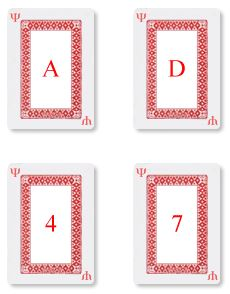
\includegraphics[width=0.8\linewidth]{figurenAuteur/loep0.jpg}
\captionof{figure}{Wasons werelberoemde kaartselectieprobleem}
\label{fig0}
\end{center}

Het inleidend voorbeeld linkt mooi aan het debat dat in de vakdidactische wiskundeliteratuur gaande is over de rol van logica in het secundair onderwijs. Er bleken wel wat aanwijzingen te bestaan dat logisch valide redeneringen maken niet zomaar een gratis bijproduct is van goed wiskunde-onderwijs als je er geen expliciete aandacht aan besteedt. Daarbovenop kan een basis logica leerlingen helpen om bepaalde bewijsvoeringen beter te begrijpen, het nut van tegenvoorbeelden in te zien... Dat is zeker zo wanneer leerlingen minder vertrouwd zijn met het lesonderwerp (Durand-Guerrier et al., 2012).  Daarnaast is logica zeer vormend: het bevindt zich op het kruispunt van filosofie en wiskunde en is volgens Aritstoteles de basis van het rationeel denken, het wetenschappelijk bewijs, de argumentatieleer (drogredeneringen/paradoxen), gevolgtrekking (causaliteit)...  Een vakgebied als informatica zou zelfs niet bestaan zonder de oerwetten der logica.

In de leerlijnen van de hervorming van het secundair onderwijs maken logica en de herwonnen aandacht voor abstractie dan ook een voorzichtige comeback bij de leerplannen wiskunde van de doorstroomfinaliteit. Tot de jaren negentig was een portie propositielogica vaste prik in het aso, voornamelijk in het vierde jaar.  Met de nieuwe eindtermen start de leerlijn logica al in de eerste graad. Leerlingen moeten in de eerste graad een onderscheid kunnen maken tussen een implicatie (als $\ldots$ dan $\ldots$) en een equivalentie ($\ldots$ als en slechts als $\ldots$). Denk maar aan tal van meetkundige eigenschappen waarin je dat verschil duidelijk kunt maken. Een bescheiden kennismaking met verzamelingenleer (unie, doorsnede, verschil) en redeneringen (bewijsjes) komt ook reeds aan bod. In de tweede graad van de doorstroom blijft de aandacht voor bewijsvoeringen bestaan, maar wordt de leerlijn logica nog iets explicieter: de leerlingen maken er kennis met de zogenaamde connectieven (en, of, niet) en stellen waarheidstabellen op. In de derde graad wordt de leerlijn logica afgerond met het afleiden van een logische uitspraak uit hypothesen door het toepassen van logische wetten. Leerlingen in een wiskunderichting maken daarnaast ook kennis met predicatenlogica, wat zeker in contexten met kwantoren (zoals bij de definitie van een limiet) erg nuttig is. 

Deze loep schreven de redacteurs Els, Filip en Hilde samen met gastauteur Alexander Holvoet. Alexander studeert aan de KU Leuven de masteropleiding wiskunde, gecombineerd met de lerarenopleiding. Hij heeft al gedurende heel zijn studietraject een bijzondere interesse voor de filosofische kanten van de koningin der wetenschappen en werkt voor zijn masterproef een cursus rond logica voor het secundair onderwijs uit. In deze loep focussen we op de tweede graad. De loep wil twee ambities waarmaken: enerzijds inspiratie bieden om met de nieuwe leerstof succesvol te starten in de klas. Zo starten we met de basis van propositielogica en waarheidstabellen, leggen we de verschillen uit tussen omgangstaal en logica en gaan we dan over op logische poorten. Anderzijds willen we ook wat dieper gaan voor de leerlingen die wat extra uitdaging kunnen gebruiken of bieden we achtergrondinformatie aan voor de leerkracht. Zo passen we logica toe in zoekmachines, leggen we de link tussen logica en bewijzen uit het ongerijmde en door contrapositie en sluiten we af in totale aporie: in de humaniora gaan we er impliciet altijd van uit dat wiskundige uitspraken waar of vals zijn. Dat is de zogenaamde \textit{wet van de uitgesloten derde} (\textit{tertium non datur}). Maar wat als we die assumptie loslaten? We geven een toegankelijk voorbeeld van waarheidstabellen in een drievoudige logica. Veel leesplezier!


\section{Propositielogica}

In deze paragraaf willen we de belangrijkste begrippen verduidelijken. Wie inspiratie zoekt voor in de klas, vindt werkteksten in de ´Onder de loep' van Uitwiskeling 27/2 (p. 9-34). 

\tussentitel{Uitspraken en proposities}
De elementaire bouwstenen van de logica zijn uitspraken of \emph{proposities}. Dat zijn zinnen die iets beweren. Bijvoorbeeld:

\begin{opsomming}                                     
\item Het is vandaag donderdag.
\item Het sneeuwt.
\item Newton is geboren in 1643.
\item 5 is kleiner dan 2.
\end{opsomming}

Van een dergelijke uitspraak kun je bepalen of ze waar is of niet. Voor bepaalde uitspraken hangt het waar zijn af van het moment waarop ze worden uitgesproken, zoals bij de eerste twee uitspraken hierboven. Van de zinnetjes hieronder kun je niet zeggen of ze waar zijn of niet.

\begin{opsomming}                                     
\item Ga zitten!
\item Zoek $x$ zodanig dat $2x+8=0$.
\item Weet jij wie de president van Amerika is?
\item 54 kilometer.
\end{opsomming}

In de logica zullen we ons bezighouden met zinnen die ofwel waar zijn ofwel niet waar. We noemen ze \emph{uitspraken} of \emph{proposities}. We zullen op een abstracter niveau omgaan met deze uitspraken en zullen de samenhang tussen verschillende uitspraken bestuderen. 

In het vervolg zullen we de letters $p$, $q$... gebruiken om uitspraken voor te stellen. Als een uitspraak waar is, dan is haar waarheidswaarde 1, als ze vals is, dan is die waarheidswaarde 0. 
 
\tussentitel{Uitspraken samenstellen}
We krijgen complexere uitspraken door de uitspraken te combineren met elkaar door gebruik te maken van logische operatoren als $\lnot$ (niet), $\land$ (en), $\lor$ (of) en $\Rightarrow$ (als ... dan ...). De logische operatoren $\lnot, \land, \lor$ en $\Rightarrow$ noemt men ook wel eens \emph{connectieven} omdat je er twee uitspraken mee bij elkaar voegt om er een nieuwe uitspraak mee te creëren. We spreken ook wel van (logische) bewerkingen.

Binnen wiskunde is het van groot belang dat we ons heel precies en ondubbelzinnig uitdrukken. We leggen daarom heel precies vast wat we met elk van de connectieven bedoelen. We geven er een definitie van door in een schema aan te geven wanneer de uitdrukking waar is en wanneer niet. Zo een schema noemen we een \emph{waarheidstabel}.

\tussentitel{Negatie}

Als $p$ een propositie is, dan noemt men $\lnot p$ (lees: niet p) de negatie (of de ontkenning) van $p$. 

De negatie van een ware propositie is een valse propositie. De negatie van een valse propositie is een ware propositie.\\

De waarheidstabel van de negatie ziet eruit als volgt:

\begin{center}
\begin{tabular}{c|c}  
$p$ & $\lnot p$\\
\hline
1 & 0\\
0 & 1
\end{tabular}
\end{center}

\tussentitel{Conjunctie}

Als $p$ en $q$ proposities zijn, dan noemt men $p \land q$ (lees: $p$ en $q$) de \emph{conjunctie} (samenvoeging) van $p$ en $q$.

De conjunctie $p\land q$ is waar als de beide proposities $p$ en $q$ waar zijn en is vals in alle andere gevallen.

De waarheidstabel van de conjunctie ziet eruit als volgt:
\begin{center}
\begin{tabular}{c|c|c}  
$p$ & $q$ & $p\land q$\\
\hline
1 & 1 & 1 \\
1 & 0 & 0\\
0 & 1 & 0\\
0 & 0 & 0
\end{tabular}
\end{center}

De propositie `het getal $\pi$ is rationaal en 5 is oneven' is dus een valse propositie. We zeggen niet dat de bewering `half waar' is.

\tussentitel{Disjunctie}

Als $p$ en $q$ proposities zijn, dan noemt men $p \lor q$ (lees: $p$ of $q$) de disjunctie van $p$ en $q$. De disjunctie $p\lor q$ is waar als minstens \'e\'en van de proposities $p$ en $q$ waar is en is vals als beide proposities vals zijn.

De waarheidstabel van de disjunctie ziet eruit als volgt:
\begin{center}
\begin{tabular}{c|c|c}  
$p$ & $q$ & $p\lor q$\\
\hline
1 & 1 & 1 \\
1 & 0 & 1\\
0 & 1 & 1\\
0 & 0 & 0
\end{tabular}
\end{center}


Wanneer de leerkracht zegt `\emph{Als huiswerk maak je oefening 5 of oefening 6}', dan zullen de meeste leerlingen slechts één oefening maken. Dat is ook wat de leerkracht bedoelt: één oefening van de twee volstaat, je moet ze zeker niet allebei maken. De \emph{of} wordt hier, zoals meestal in het dagelijks taalgebruik, \emph{exclusief} gebruikt. In de logica daarentegen is de \emph{of} een inclusieve of. Je moet in de logica geen keuze maken, je kunt ook voor beide alternatieven gaan.

Een voorbeeld uit de wiskundeles: als $a\cdot b = 0$, dan is $a = 0$ of $b = 0$. De \emph{of} is hier inclusief: minstens één van de factoren is nul, maar het kan ook zijn dat zowel $a$ als $b$ nul zijn.

In het Latijn gebruikt men \emph{aut} voor de exclusieve \emph{of} en \emph{vel} voor de inclusieve \emph{of}. Vandaar het symbool $\lor$ in de logica.


\tussentitel{Implicatie}

Als $p$ en $q$ proposities zijn, dan noemt men $p \Rightarrow q$ (lees: als $p$ dan $q$) de implicatie van $p$ naar $q$.\\

De propositie $p$ (die v\'{o}\'{o}r de pijl staat) noemen we het \emph{antecedent} en $q$ (na de pijl) noemen we het \emph{consequent}.

De implicatie $p\Rightarrow q$ is waar behalve als $p$ waar en $q$ vals is.

De waarheidstabel van de implicatie ziet er als volgt uit:
\begin{center}
\begin{tabular}{c|c|c}  
$p$ & $q$ & $p\Rightarrow q$\\
\hline
1 & 1 & 1 \\
1 & 0 & 0\\
0 & 1 & 1\\
0 & 0 & 1
\end{tabular}
\end{center}


We verduidelijken deze waarheidstabel met een voorbeeld.\\ 

Stel \\
\begin{tabular}{ll}
$p$    &  Ik ben jarig.\\
$q$   &  Ik trakteer met cake.
\end{tabular}

Dan is de implicatie \\
\begin{tabular}{ll}
$p \Rightarrow q$     &  Als ik jarig ben, trakteer ik met cake.\\
 \end{tabular}


Net zoals in de waarheidstabel onderscheiden we bij deze zin de verschillende mogelijkheden:
\begin{opsomming}

\item  Ik ben jarig ($p$ is waar) en ik trakteer met cake ($q$ is waar). In dat geval is de uitspraak $(p\Rightarrow q)$ waar.
\item Ik ben jarig ($p$ is waar) en ik trakteer niet met cake ($q$ is vals). In dat geval kom ik mijn belofte niet na en is de uitspraak $(p\Rightarrow q)$ vals. 

\item Ik ben niet jarig ($p$ is vals). In dat geval maakt het niet uit of ik trakteer of niet. In beide gevallen is $(p\Rightarrow q)$ waar.
\end{opsomming}

In de wiskunde zijn veel stellingen geformuleerd volgens een `als ... dan ...'-patroon. Zo een uitspraak is waar (en dus een stelling) indien de implicatie altijd waar is. Als we naar de waarheidstabel van de implicatie kijken, zien we dat één geval dan uitgesloten is, namelijk dat het antecedent waar is en het consequent vals. 

Zo is de uitspraak `als twee driehoeken congruent zijn, dan zijn ze gelijkvormig' een stelling. Als je wilt aantonen dat de uitspraak `als een getal deelbaar is door 12, dan is het deelbaar door 8' niet waar is, kun je dat doen door een tegenvoorbeeld te geven. Dat is een voorbeeld dat laat zien dat je het `verboden' lijntje uit de waarheidstabel wel degelijk kunt krijgen. Zo een voorbeeld is het getal 36 want 36 is deelbaar door 12 (antecedens is waar), terwijl 36 niet deelbaar door 8 is (consequens is vals). De uitspraak is dus geen stelling.  

\tussentitel{Equivalentie}

Als $p$ en $q$ proposities zijn, dan noemt men $p \Leftrightarrow q$ (lees: $p$ als en slechts als $q$) de equivalentie (gelijkwaardigheid) van $p$ en $q$. De equivalentie $p\Leftrightarrow q$ is waar als de proposities $p$ en $q$ ofwel beide waar ofwel beide vals zijn en is vals als de ene waar is en de andere vals. 

De waarheidstabel van de equivalentie ziet er als volgt uit:
\begin{center}
\begin{tabular}{c|c|c}  
$p$ & $q$ & $p\Leftrightarrow q$\\
\hline
1 & 1 & 1 \\
1 & 0 & 0\\
0 & 1 & 0\\
0 & 0 & 1
\end{tabular}
\end{center}


\tussentitel{Volgorde van de bewerkingen}

Om $3+2\cdot 6$ te berekenen in $\R$ moet je eerst de vermenigvuldiging uitvoeren en dan het verkregen product optellen bij 3.

Ook bij samengestelde proposities waarin meerdere bewerkingen met proposities voorkomen, moet je een bepaalde volgorde van de bewerkingen respecteren. 

\begin{opsomming}
\item Als er geen haakjes staan, is de volgorde: eerst $\lnot$, dan $\land$, dan $\lor$, daarna $\Rightarrow$ en ten slotte $\Leftrightarrow$.

\item Als je wilt dat de bewerkingen in een andere volgorde toegepast worden, dan moet je haakjes plaatsen.
\end{opsomming}


Ter illustratie maken we een waarheidstabel voor de propositie $\lnot p \lor q \Leftrightarrow p \Rightarrow q$. Rekening houdend met de volgorde van de bewerkingen betekent dit hetzelfde als $\big( (\lnot p) \lor q \big) \Leftrightarrow (p\Rightarrow q)$. Je hoeft de haakjes niet te schrijven, maar het is op die manier wel duidelijker. De waarheidstabel van deze propositie vind je in tabel \ref{prop1}. Uit de tabel blijkt dat deze uitspraak altijd waar is. Een dergelijke uitspraak noemen we een tautologie. We komen hier later nog op terug.

Door haakjes toe te voegen kun je een andere volgorde opdringen: $\big( \lnot (p \lor q) \big) \Leftrightarrow (p \Rightarrow q)$. De waarheidstabel van deze laatste propositie vind je in tabel \ref{prop2}. Merk op dat door het plaatsen van de haakjes de uitspraak niet langer een tautologie is.

\end{multicols}
\begin{table}[h]
\begin{center}
\begin{tabular}{c|c|c|c|c|c}  
$p$ & $q$ & $\lnot p$ & $\lnot p \lor q$ & $p\Rightarrow q$ & $\big( (\lnot p) \lor q \big) \Leftrightarrow (p\Rightarrow q)$\\
\hline
1 & 1 & 0 & 1 & 1 & 1\\
1 & 0 & 0 & 0 & 0 & 1\\
0 & 1 & 1 & 1 & 1 & 1\\
0 & 0 & 1 & 1 & 1 & 1
\end{tabular}
\caption{Waarheidstabel van $\lnot p \lor q \Leftrightarrow p \Rightarrow q$} \label{prop1}
\end{center}
\end{table}


\begin{table}[h]
\begin{center}
\begin{tabular}{c|c|c|c|c|c}  
$p$ & $q$ & $p\lor q$ & $\lnot (p\lor q)$ & $p \Rightarrow q$ & $\big( \lnot (p \lor q) \big) \Leftrightarrow (p \Rightarrow q)$\\
\hline
1 & 1 & 1 & 0 & 1 & 0\\
1 & 0 & 1 & 0 & 0 & 1\\
0 & 1 & 1 & 0 & 1 & 0\\
0 & 0 & 0 & 1 & 1 & 1
\end{tabular}
\caption{Waarheidstabel van $\big( \lnot (p \lor q) \big) \Leftrightarrow (p \Rightarrow q)$} \label{prop2}
\end{center}
\end{table}
\begin{multicols}{2}




\section{Logicataal versus omgangstaal}



%\subsection{Typ hier de deelparagraaftitel}
%\tussentitel{Typ hier de tussentitel}

Onze gewone taal is rijker dan de formele taal van de propositielogica. Niet alle nuances uit de omgangstaal kunnen met propositielogica worden weergegeven. 

We geven enkele voorbeelden.

Hierboven is al opgemerkt dat er een verschil is in het gebruik van het woord `of'. Wanneer je in een gewone taal, zoals het Nederlands, zegt \textsl{Voor mij past deze vergadering op dinsdag- of donderdagnamiddag}, dan bedoel je \textsl{De vergadering kan gepland worden ofwel op dinsdagnamiddag ofwel op donderdagnamiddag}. Je bedoelt natuurlijk niet dat je twee keer wilt vergaderen: op dinsdag- en op donderdagnamiddag. In een gewone taal heeft het woord \textsl{of} meestal een \emph{exclusieve} betekenis. In de logica betekent het woord \textsl{of}: ofwel het ene ofwel het andere ofwel beide samen. Het woord \textsl{of} heeft hier dus een \emph{inclusieve} betekenis.

In de propositielogica geldt de commutatieve wet voor de conjunctie: $p\land q$ is logisch equivalent met $q\land p$. Dit kun je ook in de omgangstaal gebruiken.\\ \textsl{Emma gaat naar het feest en Ilyes blijft thuis} betekent hetzelfde als \textsl{Ilyes blijft thuis en Emma gaat naar het feest.} In de gewone omgangstaal kun je dit soort zinnen echter niet altijd omdraaien. De zin
\textsl{Leon trekt zijn sokken uit en gaat naar bed} heeft niet dezelfde betekenis als
\textsl{Leon gaat naar bed en trekt zijn sokken uit.} In de omgangstaal gaat het vaak om een opeenvolging van gebeurtenissen die na elkaar plaats hebben en dat tijdsverloop kunnen we in de propositielogica niet weergeven. Ook gelijktijdigheid kunnen we niet weergeven met propositielogica. Zo kun je bijvoorbeeld met een conjunctie niet uitdrukken dat Dimitri Thivaios en Michael Thivaios, die het beroemde DJ-duo Dimtri Vegas en Like Mike vormen, samen op Tomorrowland hebben opgetreden. Je zult dit moeten schrijven als $p \land q$ waarbij $p$ betekent \textsl{Dimitri heeft opgetreden op Tomorrowland} en $q$ \textsl{Michael heeft opgetreden op Tomorrowland}.

Vaak treden er ook nuanceverschillen op bij de vertaling van samengestelde zinnen naar logicataal. De zin \textsl{Kadja is slim, maar ze gaat geen wiskunde studeren} kun je schrijven met propositielogica als $s\land w$. De propositie $s$ is hierbij \textsl{Kadja is slim} en $w$ betekent \textsl{Kadja volgt de masteropleiding wiskunde niet}. Toch ben je informatie verloren. De oorspronkelijke uitspraak drukt ook de verwachting uit dat wie slim is wiskunde gaat studeren.

Veel concrete `als dan'-uitspraken uit het dagelijks leven voldoen niet aan de logische regels
van een wiskundige implicatie. Een standaardvoorbeeld is \textsl{Als je braaf bent, dan krijg je
een snoepje}. Deze uitspraak lijkt een implicatie, maar wanneer je dit bekijkt door een propositielogicabril dan is dat geen implicatie. We gaan er immers van uit dat bovenstaande zin ook inhoudt dat je geen snoepje krijgt als je niet braaf bent. De uitspraak \textsl{Als je braaf bent, dan krijg je een snoepje} wordt dus eigenlijk als een equivalentie bedoeld. Dat doen we in ons dagelijks leven vaak bij taalgebonden uitspraken: we maken geen onderscheid tussen implicatie en equivalentie en benadrukken de equivalentie niet. In wiskundetaal doen we dat dikwijls wel door constructies te gebruiken met `als en slechts als'. Al houden sommige definities ook wel een verborgen equivalentie in. Bekijk de definitie \textsl{Als de vier zijden van een vierhoek even lang zijn, dan noemen we die vierhoek een ruit}. Hier bedoelen we meteen ook dat we andere vierhoeken geen ruit noemen. Ook binnen wiskunde wordt de logica dus soms informeel gebruikt.

Door de nuanceverschillen met onze omgangstaal is het voor leerlingen niet altijd eenvoudig om de vertaling van die  gewone taal naar de formele taal van de logica te maken. De volgende lesactiviteit laat enkele van de moeilijkheden zien en kan aanleiding geven tot een klasdiscussie over de beperkingen van propositielogica t.o.v. de omgangstaal. Merk hierbij op dat er soms meerdere antwoorden kunnen zijn. Je bespreekt dan best de mogelijke interpretaties. De vertaling van de beweringen is niet gemakkelijk. Het is daarom goed om de verschillende antwoorden aan het bord te verzamelen en die één voor één klassikaal te bespreken.

We merken op dat je de discussie over de nuances in onze omgangstaal ook zou kunnen gebruiken als aanleiding om de logische connectieven in te voeren. Als je bijvoorbeeld enkele zinnen met een `of' met verschillende betekenis toont, wordt duidelijk dat er nood is aan een formele inclusieve of. De volgorde zou dus voor sommige problemen met de omgangstaal omgedraaid kunnen worden: eerst enkele goed gekozen zinnen in omgangstaal/wiskundige taal vergelijken en pas dan formaliseren.

\end{multicols}
\beginwerktekst{Van omgangstaal naar propositielogica}

De overgang van omgangstaal naar propositielogicataal kun je meestal niet maken door eenvoudigweg de atomaire zinnen te herschrijven met een letter en het voegwoord `en' te vervangen door $\land$,  `of' te vervangen door $\lor \ldots$ We gebruiken in het Nederlands immers veel meer voegwoorden (echter, daarentegen, maar, tenzij, mits, want, hoewel $\ldots$). De nuances die we met die voegwoorden kunnen maken, zijn niet altijd precies met propositielogicataal weer te geven waardoor er betekenisverschillen kunnen ontstaan. Deze problemen kun je ook hebben bij wiskundetaal die in Nederlandse zinnen is geformuleerd.

Vertaal de volgende zinnen zo adequaat mogelijk naar propositielogica. Is de betekenis helemaal dezelfde gebleven? 


\begin{werktekstoef}
\item{Sofia noch Lars hebben hun huiswerk al gemaakt, maar toch gaan zij naar het feestje.\\ Gebruik de volgende vertaalsleutel: $s=$ Sofia heeft haar huiswerk gemaakt, $l=$ Lars heeft zijn huiswerk gemaakt, $f=$ ze gaan naar het feestje.}

\emph{De enige manier waarop je dit kunt vertalen is $\lnot s \land \lnot l \land f$. Dit heeft echter niet dezelfde betekenis als de gegeven bewering. Die laatste houdt namelijk ook een waardeoordeel in (ze verdienen het niet om  naar het feestje te gaan). Dat kunnen we niet bekomen met propositielogica. %Ook het woordje `al' vinden we niet meer terug (ze zouden hun huiswerk nadien nog kunnen maken; op een later moment is het dus misschien $s \land l \land f)$).
}


\item{We laten je ten laatste 25 april weten of je met onze organisatie op sportkamp kan, mits je het aanvraagformulier tijdig indient.\\ Gebruik hierbij als sleutel: $w=$ we laten je weten of je mee op kamp kan, $t=$ je dient het aanvraagformulier tijdig in.}

\emph{De bewering houdt zeker het volgende in: $t\Rightarrow w$. Of de bewering ook betekent $\lnot t \Rightarrow \lnot w$ kun je in vraag stellen. Vaak bedoelt men dat wel, al staat het er niet letterlijk. Vaak bedoelt men met de bewering een equivalentie: $t\Leftrightarrow w$. Je kunt hierover discussiëren: er zijn ook argumenten om te zeggen dat $\lnot t \Rightarrow \lnot w$ niet juist is. Er wordt nergens gezegd wat er gedaan wordt als je het aanvraagformulier niet tijdig indient. Het kan zijn dat men je dan toch nog voor 25 april verwittigt of dat er bijvoorbeeld een (geheime) marge is: tot twee dagen later wordt het formulier ook nog aanvaard.}

\item{Kaat gaat alleen naar school als ze zin heeft.\\ Gebruik hierbij de sleutel: $s=$ Kaat gaat naar school, $z=$ Kaat heeft zin in school.}

\emph{Geldt $z \Rightarrow s$? Eigenlijk niet, want dat zou betekenen dat Kaat altijd naar school gaat als ze zin heeft en dat staat er niet (al kun je hier over discussiëren: de alleen-als-constructie kan ook gebruikt zijn om te benadrukken dat ze naar school gaat als en alleen als ze zin heeft).\\ Zeker staat er: als Kaat geen zin heeft, dan gaat ze niet naar school. Dit betekent: $\lnot z \Rightarrow \lnot s$. Dit is equivalent met $s\Rightarrow z$. Anders gezegd: als je vaststelt dat Kaat naar school gaat, dan weet je wel zeker dat ze zin heeft. Je kunt dit gemakkelijk verifiëren met waarheidstabellen. De gelijkwaardigheid van $\lnot z \Rightarrow \lnot s$ en $s\Rightarrow z$ noemt men de wet van de contrapositie.}


\item{Liv gaat altijd naar school, tenzij ze naar de dokter moet.\\ Gebruik de volgende vertaalsleutel: $s =$ Liv gaat naar school, $d =$ Liv moet naar de dokter.}

\emph{Uit de bewering volgt: als Liv naar de dokter moet, dan gaat ze niet naar school. Met propositielogica: $d\Rightarrow \lnot s$. Dat is echter  niet genoeg. De gegeven bewering houdt ook in dat Liv in alle andere gevallen wél naar school gaat. Dit betekent: als Liv niet naar school is, dan weet je dat ze naar de dokter is. Anders gezegd: $\lnot s \Rightarrow d$. Besluit: de bewering kan vertaald worden als $d\Leftrightarrow \lnot s$.}


%\item{Bezwaarschriften tegen het bouwproject worden niet in behandeling genomen, tenzij deze tijdig zijn ingeleverd.\\ Gebruik de volgende sleutel: $b =$ de bezwaarschriften worden in behandeling genomen, $t =$ de bezwaarschriften zijn tijdig ingeleverd.}

\item{Ilyes laat geen verstek gaan voor de middagsportactiviteit, behalve als hij echt ziek is.\\ Sleutel: $v =$ Ilyes laat verstek gaan voor de middagsportactiviteit, $z =$ Ilyes is echt ziek.}

\emph{De bewering kan ook als volgt geformuleerd worden: als Ilyes verstek laat gaan, dan moet hij wel echt ziek zijn. Dit betekent: $v \Rightarrow z$. Merk op dat je dit ook kunt formuleren als: als Ilyes niet echt ziek is, dan laat hij geen verstek gaan ($\lnot z \Rightarrow \lnot v$). Dit is de contrapositie van $v \Rightarrow z$. Anderzijds kun je erover discussiëren of er ook staat: als Ilyes echt ziek is, dan laat hij verstek gaan. Sommigen zullen vinden van wel, anderen leiden dit misschien niet af uit de gegeven uitspraak. Of er geldt $z \Rightarrow v$ en er dus eigenlijk een equivalentie staat (zoals in de vorige oefening), is hier dus niet helemaal duidelijk.}


%\item{Ik heb niet gezegd dat je niet naar school mag.\\ Sleutel: $p=$ ik heb gezegd dat je naar school mag.}

%\emph{Dit is een dubbele negatie. Je kunt dit vertalen als $\lnot (\lnot p)$. In propositielogica is dit logisch equivalent met $p$. In de omgangstaal is er echter een nuanceverschil. Met het gebruik van `niet' wil je extra benadrukken wat je niet gezegd hebt. De uitspraak `Ik heb gezegd dat je naar school mag' houdt een expliciete toelating in om naar school te gaan. Met de dubbele negatie geef je aan dat je een meer impliciete toelating hebt gegeven.}

\item{Een voorbeeld uit wiskunde.\\ In een rechthoekige driehoek $ABC$ is het kwadraat van de lengte van de hoogtelijn op de schuine zijde gelijk aan het product van de lengtes van de stukken waarin die hoogtelijn de schuine zijde verdeelt.\\ Sleutel: $r=$ een driehoek $ABC$ is rechthoekig, $h=$ het kwadraat van de lengte van de hoogtelijn op de schuine zijde is gelijk aan het product van de lengtes van de stukken waarin die hoogtelijn de schuine zijde verdeelt. }

\emph{De vertaling naar propositielogica is $r\Rightarrow h$. We bedoelen hier dat de uitspraak geldt voor alle rechthoekige driehoeken. Sommige leerlingen zouden de gegeven zin echter ook kunnen interpreteren als `Er is (of er bestaat) een rechthoekige driehoek $ABC$ waarvoor $\ldots$'}

\item{Een strikt positief reëel getal heeft twee tegengestelde vierkantswortels.\\ Zoek zelf een vertaalsleutel.}

\emph{Stel $p=$ een getal is een strikt positief reëel getal en $t=$ het getal heeft twee tegengestelde vierkantswortels. Dan hebben we: $p\Rightarrow t$. Ook hier mag je de zin niet interpreteren als `Er bestaat een strikt positief reëel getal met twee tegengestelde vierkantswortels'. De eigenschap geldt voor alle strikt positieve reële getallen of nog $\forall a \in \R_0^+:$ $a$ heeft twee tegengestelde vierkantswortels $\sqrt{a}$ en $-\sqrt{a}$.}


% oefeningomgeving stoppen om tussentekst in te voegen als dat nodig is
\end{werktekstoef}  
\eindewerktekst

\begin{multicols}{2}

Er zijn logische talen ontwikkeld die met bepaalde beperkingen van de propositielogica kunnen omgaan. In de derde graad staat voor sommige leerlingen een uitbreiding naar predicatenlogica op het programma. Je hebt bijvoorbeeld ook nog temporele logica, waarin verschillen in tijd kunnen worden uitgedrukt. De klassieke propositielogica is tweewaardig of binair: er zijn twee logische waarden 0 of 1. Meerwaardige logica's daarentegen hebben meer dan twee logische waarden. In paragraaf 8 bespreken we kort zo'n uitbreiding.


\section{Proposities onderzoeken met waarheidstabellen}

Zoals je in de voorbeelden hierboven al zag, kun je met een waarheidstabel onderzoeken wanneer een gegeven samengestelde propositie waar is en wanneer ze vals is. In de lesactiviteit hieronder laten we de leerlingen hier zelf mee experimenteren.

\end{multicols}
\newpage

\beginwerktekst{Waarheidstabellen, logische wetten en tautologieën}

Met waarheidstabellen kun je de waarheidswaarde van logische uitspraken onderzoeken. Je stelt dan een tabel op met ruimte voor alle mogelijke waarheidswaarden van de propositieletters. Vervolgens bouw je stap voor stap de samengestelde proposite op en bepaal je hiervan de waarheidswaarde. Ten slotte combineer je de stukjes en stel je de waarheidswaarde van de hele formule op. Bij wijze van inleiding doen we dit voor de uitdrukking $q\land \lnot p \Rightarrow r$. Dit is een samengestelde propositie met drie propositieletters. In de waarheidstabel moet je dan $2^3=8$ lijnen met de verschillende mogelijkheden voor $p$, $q$ en $r$ voorzien.

\begin{center}
\begin{tabular}{c|c|c|c|c|c}  
$p$ & $q$ & $r$ & $\lnot p$ & $q\land \lnot p$ & $q\land \lnot p \Rightarrow r$\\
\hline
1 & 1 & 1 &  &  & \\
1 & 1 & 0 &  &  & \\
1 & 0 & 1 &  &  & \\
1 & 0 & 0 &  &  & \\
0 & 1 & 1 &  &  & \\
0 & 1 & 0 &  &  & \\
0 & 0 & 1 &  &  & \\
0 & 0 & 0 & 1 & 0 & 1
\end{tabular}
\end{center}

\begin{werktekstoef}
\item{Vul de waarheidstabel verder aan.}
\end{werktekstoef}

Twee logische uitspraken kunnen gelijkwaardig zijn of niet. Dat is niet altijd op het eerste gezicht te zien. De eenvoudigste manier om dit na te gaan is van beide formules een waarheidstabel op te stellen en ze te vergelijken. Indien de twee formules dezelfde waarheidswaarde hebben voor de verschillende situaties, dan zijn ze equivalent. 

\begin{werktekstoef}
\setcounter{enumi}{1} 
\item{Stel de waarheidstabel op voor $\lnot (\lnot p)$}

\emph{De waarheidstabel is:}
\end{werktekstoef}
\begin{center}
\begin{tabular}{c|c|c}  
$p$ & $\lnot p$ & $\lnot (\lnot p)$\\
\hline
1 & 0 & 1\\
0 & 1 & 0
\end{tabular}
\end{center}

\begin{werktekstoef}
\setcounter{enumi}{2} 
\item{Vergelijk de eerste en de laatste kolom in de waarheidstabel. Wat stel je vast?}

\emph{Omdat de eerste en de derde kolom identiek zijn, mag je zeggen dat $p$ en $\lnot (\lnot p)$ equivalent zijn.}
\end{werktekstoef}

\begin{werktekstoef}
\setcounter{enumi}{3} 
\item{Stel de waarheidstabel op bij de formule $p \Leftrightarrow \lnot (\lnot p)$. Wat stel je vast?}

\emph{Je kunt gewoon een extra kolom toevoegen aan je vorige tabel. Dit geeft:}

\begin{center}
\begin{tabular}{c|c|c|c}  
$p$ & $\lnot p$ & $\lnot (\lnot p)$ & $p \Leftrightarrow \lnot (\lnot p)$\\
\hline
1 & 0 & 1 &1\\
0 & 1 & 0 &1
\end{tabular}
\end{center}

\emph{De propositie $p \Leftrightarrow \lnot (\lnot p)$ is altijd waar. Je kunt dit in de waarheidstabel heel snel zien doordat in de laatste kolom overal `1' staat.}
\end{werktekstoef}

Een logische uitspraak die altijd waar is, noemen we een \emph{tautologie}: de propositie $p \Leftrightarrow \lnot (\lnot p)$ is dus een tautologie.

Met de techniek van de waarheidstabellen kunnen we enkele bekende logische wetten aantonen. 

\begin{opsomming}
\item $p \lor \lnot p$ (wet van de uitgesloten derde)
\item $(p \Rightarrow q) \Leftrightarrow (\lnot q \Rightarrow \lnot p)$ (wet van de contrapositie)
\item $(p \Rightarrow q) \Leftrightarrow (\lnot p \lor q)$ (implicatie schrijven met $\lor$ en $\lnot$)
\item $(p \land \lnot p) \Rightarrow q$ (uit een onwaarheid kun je alles besluiten) 
\end{opsomming}

\begin{werktekstoef}
\setcounter{enumi}{4} 
\item{Stel voor elk van de wetten hierboven de waarheidstabel op en ga na dat het tautologieën zijn.}

\item{Pas de wet van de contrapositie toe op de stelling: `als $2^p -1$ priem is, is $p$ priem.'}

\emph{Als $p$ niet priem is, is $2^p -1$ niet priem.}

\item{Herformuleer de implicatie `als $2^p -1$ priem is, is $p$ priem' met behulp van de negatie en disjuctie.}

\emph{$2^p -1$ niet priem of $p$ is priem.}
\end{werktekstoef}

\begin{center}
     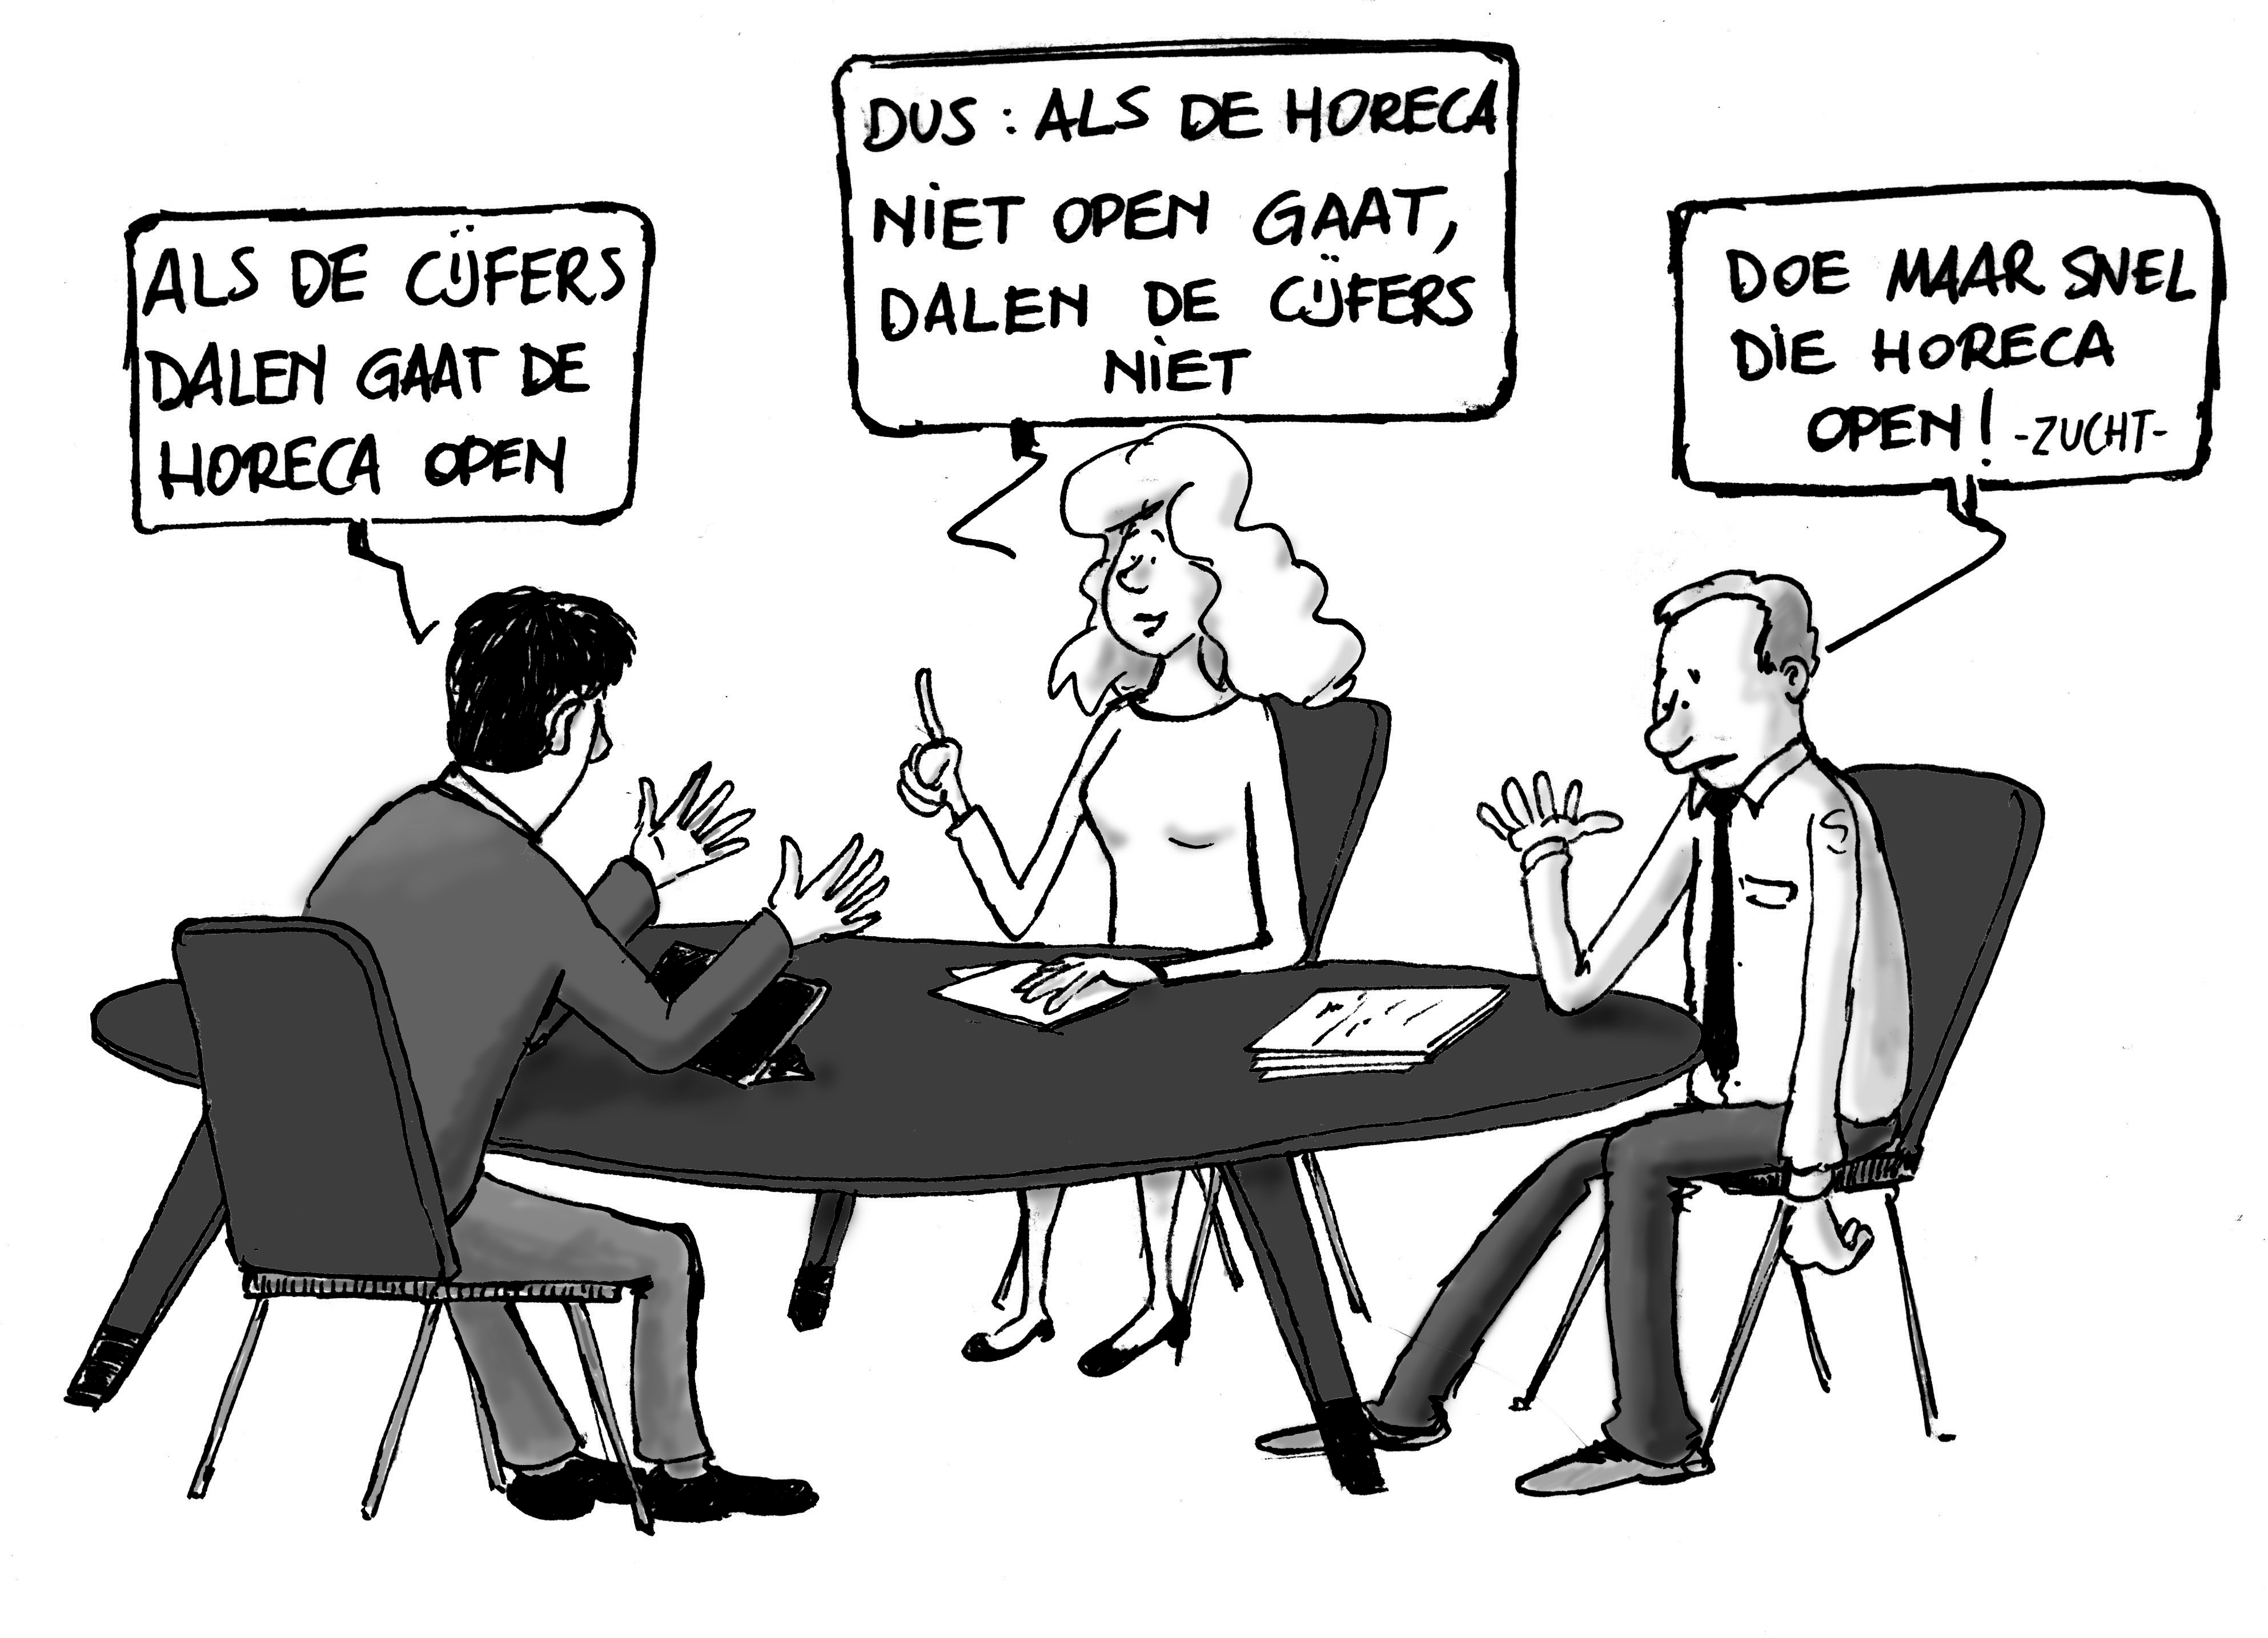
\includegraphics[width=0.9\linewidth]{tekeningenKurt/Kurt contrapositie.jpg}
\end{center}
   
   
\eindewerktekst



\begin{multicols}{2}

\section{Toepassing in digitale technieken}

Ondanks, of misschien wel net dankzij, de beperkingen die de tweewaardige propositielogica heeft ten aanzien van onze natuurlijke taal, wordt deze logica massaal toegepast in digitale systemen zoals computers, smartphones, digitale televisie, thermostaten $\ldots$ Deze systemen zijn niet meer weg te denken uit onze maatschappij, integendeel: het belang ervan neemt nog toe. De productie van geïntegreerde schakelingen (of elektronische chips) en microprocessoren wordt steeds goedkoper en het aantal transistoren op zo'n chip neemt nog steeds toe. Processoren vormen de kern van onze computers. Bij alles wat je met een computer doet (surfen op het internet, muziek luisteren, iets aanklikken $\ldots$) zijn er berekeningen nodig en die worden door de processor verwerkt. Deze processor bestaat uit allerlei digitale schakelingen. Deze digitale schakelingen werken met elektrische stromen en spanningen. Hierbij worden er twee spanningsniveaus onderscheiden: een laag niveau (aangegeven met de letter L, Low) en een hoog niveau (letter H, High). Meestal laat men met het lage niveau de waarde 0 en met het hoge niveau de waarde 1 overeenkomen. De waarden van L en H worden door de fabrikant van de chips bepaald. Vaak is een hoge spanning een spanning in de buurt van $5$ V en een lage spanning komt dan overeen met een waarde die ongeveer $0$ V is. De meest moderne chips zijn een stuk energiezuiniger en hebben een hoge spanning van bijvoorbeeld $1,8$ V. In zulke digitale schakeling wordt gebruik gemaakt van logische poorten die één of meerdere inkomende signalen omzetten in één nieuw, uitgaand signaal. Deze logische poorten worden met elkaar gecombineerd waardoor complexe schakelingen kunnen worden gerealiseerd (de output van de ene poort wordt bijvoorbeeld gebruikt als input van een volgende poort). We bekijken eerst het concept van logische schakelingen en focussen daarna op logische poorten.


\subsection{Logische schakelingen}

De meeste leerlingen kennen het concept van een elektrische kring met schakelingen al uit de lessen techniek. Een schakeling kan schematisch voorgesteld worden zoals bijvoorbeeld in figuur \ref{serie}. Naast deze schematische voorstelling kunnen we zo'n schakeling ook voorstellen met een waarheidstabel (zie bijvoorbeeld tabel \ref{tabelserie}). 

De eenvoudigste component van een schakeling is een schakelaar met twee standen: open (wat we in de waarheidstabel meestal aangeven met $0$) en gesloten (waarde in de tabel is dan meestal $1$). Voor de duidelijkheid beelden we deze schakelaars in schematische voorstellingen altijd open af.  Op eenzelfde wijze kunnen we andere componenten uit een schakeling, zoals bijvoorbeeld een lamp, in de schakeling opnemen: een lamp die uit is, geven we in de waarheidstabel aan met $0$, een brandende lamp krijgt waarde $1$.

%In een schakeling kan een processor meerdere inputs ontvangen, maar slechts één output produceren. D.w.z. dat er steeds meerdere schakelaars kunnen zijn, maar slechts één lamp. 

\tussentitel{Enkele veel voorkomende basisschakelingen}

Figuur \ref{serie} geeft een schematische voorstelling van een serieschakeling van twee schakelaars, $A$ en $B$. De lamp is aangeduid met de letter $L$ en met pictogram $\bigotimes$. De spanningsbron of voeding wordt hier aangeduid met een cirkel met de letter $U$ ernaast.

Op dezelfde manier geeft figuur \ref{parallel} een vereenvoudigde voorstelling van een parallelschakeling van twee schakelaars.


Het is een mooie oefening om voor elk van deze schakelingen een waarheidstabel te maken, net zoals we dat doen voor proposities. In deze tabel worden de toestanden van de schakelaars en de lamp met een 0 of een 1
aangegeven. Aan elke rij kunnen we een betekenis koppelen.

Voor de serieschakeling (zie figuur \ref{serie}) ziet de waarheidstabel er als volgt uit:

\begin{center}
\begin{tabular}{c|c|c|l}  
$A$ & $B$ & $L$ & betekenis\\
\hline
1 & 1 & 1 & schakelaars gesloten, lamp aan\\
1 & 0 & 0 & $A$ gesloten, $B$ open, lamp uit\\
0 & 1 & 0 & $A$ open, $B$ gesloten, lamp uit\\
0 & 0 & 0 & schakelaars open, lamp uit
\end{tabular}
\captionof{table}{Waarheidstabel bij de serieschakeling}
\label{tabelserie}
\end{center}

We stellen vast dat dit dezelfde waarheidstabel is als die van de conjunctie (en). We spreken dan ook van de logische AND-schakeling.

We kunnen deze AND-schakeling ook noteren met een zogenaamde logische vergelijking: 
\begin{center}
    $L=A\cdot B$.
\end{center}
De keuze voor het product in de logische vergelijking voor de AND-schakeling is duidelijk omdat in de waarheidstabel de waarde voor $L$ telkens gevonden kan worden door de waarden van $A$ en $B$ te vermenigvuldigen. Al gaat het in die tabel natuurlijk niet om een gewone vermenigvuldiging.


\begin{center}
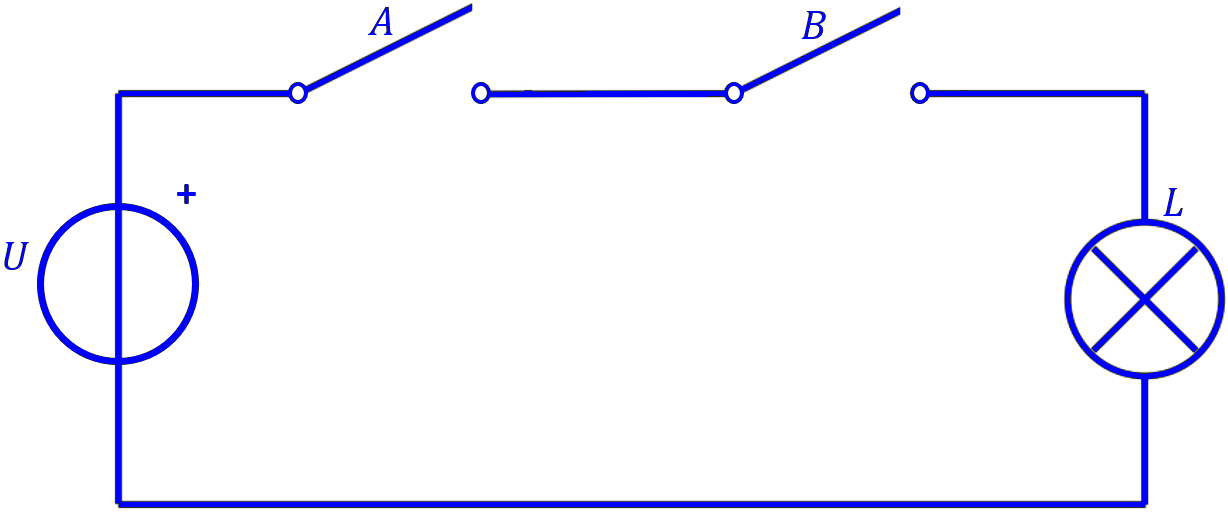
\includegraphics[width=0.8\linewidth]{figurenAuteur/serieschakeling.jpg}
\captionof{figure}{De logische AND-schakeling}
\label{serie}
\end{center}


De waarheidstabel voor de parallelschakeling (zie figuur \ref{parallel}) is de volgende:

\begin{center}
\begin{tabular}{c|c|c|l}  
$A$ & $B$ & $L$ & betekenis\\
\hline
1 & 1 & 1 & schakelaars gesloten, lamp aan\\
1 & 0 & 1 & $A$ gesloten, $B$ open, lamp aan\\
0 & 1 & 1 & $A$ open, $B$ gesloten, lamp aan\\
0 & 0 & 0 & schakelaars open, lamp uit
\end{tabular}
\captionof{table}{Waarheidstabel bij de parallelschakeling}
\label{tabelparallel}
\end{center}

We herkennen de waarheidstabel van de disjunctie (of) en we spreken van de logische OR-schakeling.

We noteren deze OR-schakeling met de logische vergelijking 
\begin{center}
    $L=A + B$.
\end{center}
De keuze voor de som in de logische vergelijking voor de OR-schakeling lijkt ook hier weer logisch al is het duidelijk dat het in de tabel niet om een gewone som gaat.
Je kunt dit als een som interpreteren door 0 te zien als niets en 1 als iets. Dan is het gemakkelijk te onthouden:
\begin{align*}
\text{iets} + \text{iets} &= \text{iets,}\\
\text{iets} + \text{niets} &= \text{iets,}\\
\text{niets} + \text{iets} &= \text{iets,}\\
\text{niets} + \text{niets} &= \text{niets.}
\end{align*}


\begin{center}
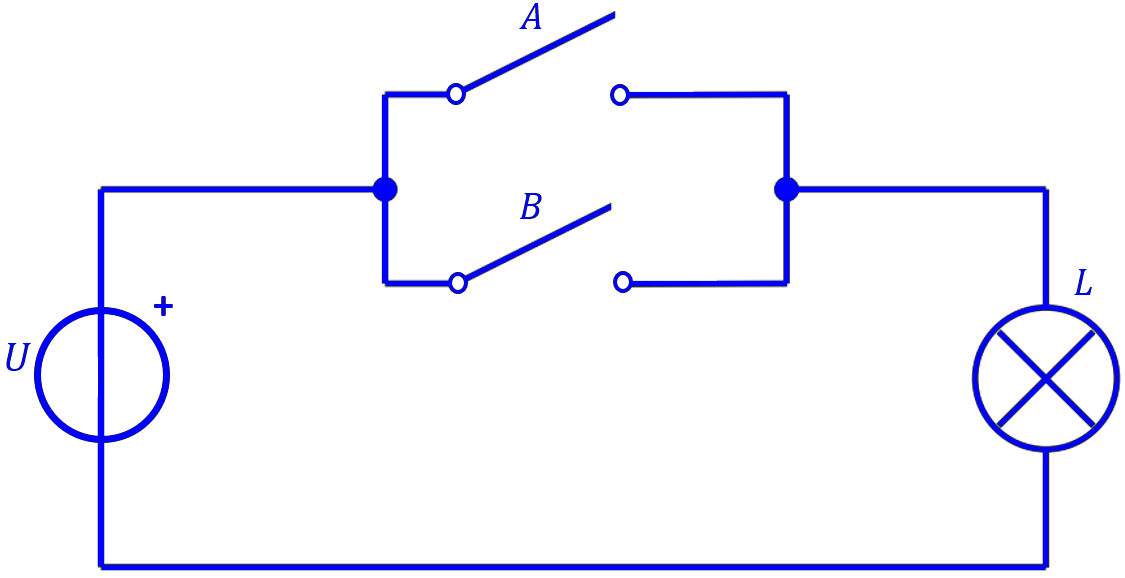
\includegraphics[width=0.8\linewidth]{figurenAuteur/parallelschakeling.jpg}
\captionof{figure}{De logische OR-schakeling}
\label{parallel}
\end{center}



%Vaak gebruiken informatici andere manieren om dit te noteren (o.a. met Boole-algebra), maar daar gaan we hier niet op in. Wij houden het bij onze eerder ingevoegde notaties uit de propositielogica.

De schakelaars die we hierboven gebruikten, kregen waarde $0$ als ze open zijn. Dit wordt gedaan bij schakelaars die in ruststand open zijn (we noemen zo'n schakelaar \textit{normally open}). De waarheidstabel bij een schakeling met één zo'n schakelaar $A$ en een lamp $L$ is nogal triviaal:

\begin{center}
\begin{tabular}{c|c|l}  
$A$ & $L$ & betekenis\\
\hline
1 & 1 & schakelaar $A$ gesloten, lamp aan\\
0 & 0 & $A$ open, lamp uit
\end{tabular}
\captionof{table}{Waarheidstabel van een normally open schakelaar}
\label{tabelnormallyopen}
\end{center}

De logische vergelijking die bij deze schakeling hoort is $L=A$.

We willen nu de tabel maken van $\lnot A$ of van de NOT-schakeling. Daarvoor hebben we een schakelaar nodig die in ruststand gesloten is en dan waarde $0$ krijgt. Als de schakelaar open is, krijgt die de waarde $1$. Zo'n schakelaar noemen we een \textit{normally closed} schakelaar.

In figuur \ref{not} is een schakeling getekend met een normally closed schakelaar. Als de schakelaar gesloten is (ruststand, waarde $0$), brandt de lamp en omgekeerd.

\begin{center}
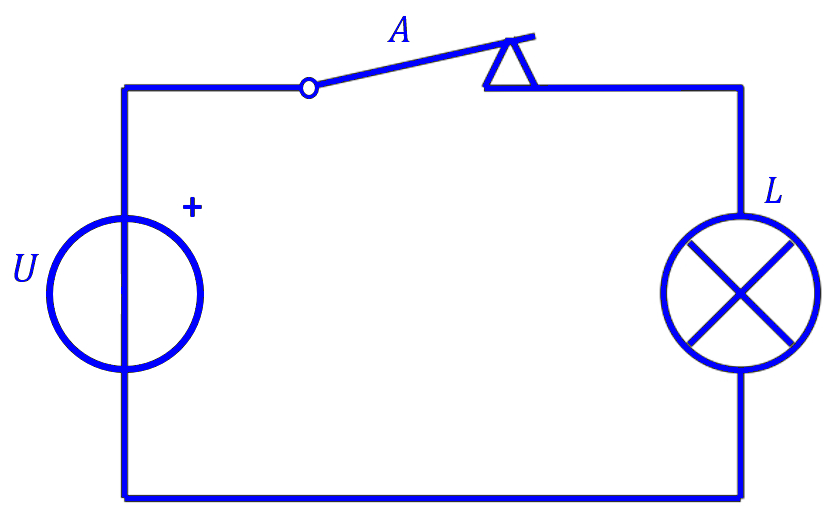
\includegraphics[width=0.55\linewidth]{figurenAuteur/not.jpg}
\captionof{figure}{De logische NOT-schakeling}
\label{not}
\end{center}


Dit levert volgende waarheidstabel, de tabel voor de negatie:

\begin{center}
\begin{tabular}{c|c|l}  
$A$ & $L$ & betekenis\\
\hline
1 & 0 & schakelaar $A$ open, lamp uit\\
0 & 1 & $A$ gesloten, lamp aan
\end{tabular}
\captionof{table}{Waarheidstabel van een normally closed schakelaar}
\label{tabelnormallyclosed}
\end{center}

We herkennen de waarheidstabel van de negatie en spreken daarom van de NOT-schakeling.
De logische vergelijking van de NOT-schakeling is 
\begin{center}
    $L=\overline{A}.$
\end{center}

In de logische vergelijkingen gebruikt men soms ook de notaties uit de propositielogica. Men noteert dan $L=A\land B$ voor de AND-schakeling, $L=A\lor B$ voor de OR-schakeling en $L=\lnot A$ voor de NOT-schakeling.

Het is interessant om in de klas te vragen of de leerlingen apparaten kennen met AND-, OR- of NOT-schakelingen. Misschien kennen/bedenken sommige leerlingen er wel.

\begin{center}
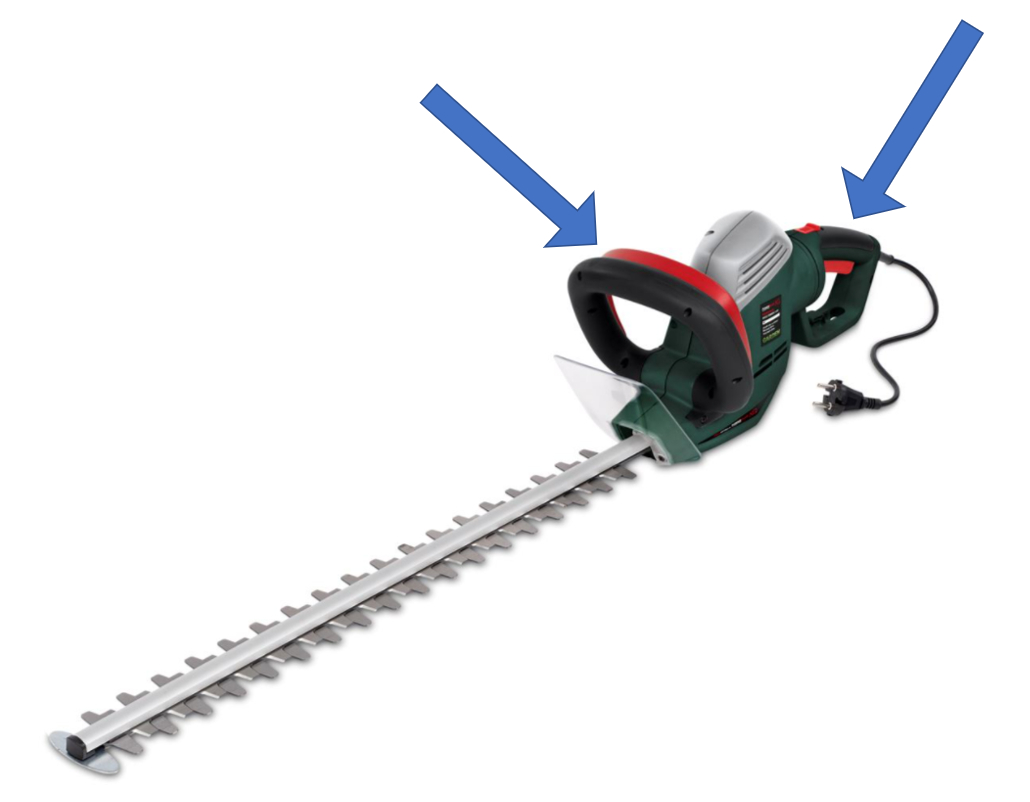
\includegraphics[width=\linewidth]{figurenAuteur/haagschaar.jpg}
\captionof{figure}{Haagschaar met twee schakelaars om de motor in te schakelen}
\label{haag}
\end{center}

De AND-schakeling komt typisch voor bij een haagschaar (of ook bij sommige grasmaaiers of verticuteermachines). Een haagschaar heeft meestal twee aan-uit-schakelaars. Op figuur \ref{haag} zijn deze met blauwe pijlen aangeduid. De ene schakelaar is een tuimelschakelaar (die aan of uit geklikt moet worden). De andere schakelaar is een hendel die je moet blijven indrukken opdat de motor van de haagschaar zou blijven werken. Van zodra je die hendel loslaat, valt de haagschaar stil.

De schakelaars om een bus te laten stoppen, vormen een typisch voorbeeld van een OR-schakeling. Om de bus te laten stoppen, moet minstens één van de vele stopknoppen in de bus worden ingedrukt.

\begin{center}

\includegraphics[width=0.8\linewidth]{figurenAuteur/busstop.jpg}
\captionof{figure}{Stopknop in een bus}
\label{bus}
\end{center}

Een ander voorbeeld van een OR-schakeling vind je bij spelletjes met meerdere spelers waarbij zo snel mogelijk op een knop moet worden gedrukt.

\begin{center}
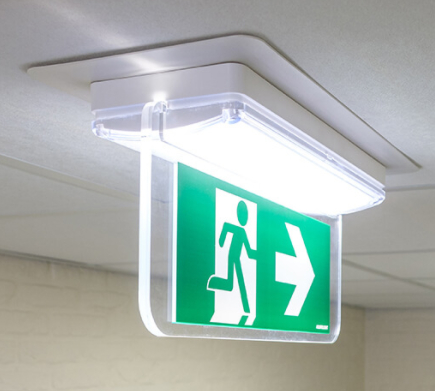
\includegraphics[width=0.8\linewidth]{figurenAuteur/noodlicht.jpg}
\captionof{figure}{Noodverlichting aan het plafond}
\label{nood}
\end{center}

De NOT-schakeling komt voor bij de gekende noodverlichting in gebouwen: als de stroom uitvalt, gaat de noodverlichting aan. 

\tussentitel{Logische schakelingen combineren} 
De AND-, OR- en NOT-schakelingen kun je nu op allerlei manieren combineren.
 
In figuur \ref{compl1} zie je hoe drie schakelaars kunnen worden gebruikt om het licht te
controleren op een meer complexe manier. Je kunt met je leerlingen de waarheidstabel van deze schakeling zoeken (zie tabel \ref{tabelORAND}). Met de notaties uit de propositielogica zouden we deze schakeling kunnen noteren als $(A\lor B)\land C$. Het licht brandt als $C$ gesloten is en tegelijkertijd minstens één van de schakelaars $A$ of $B$ gesloten is. We spreken hier van de OR-AND-schakeling. 

\begin{center}
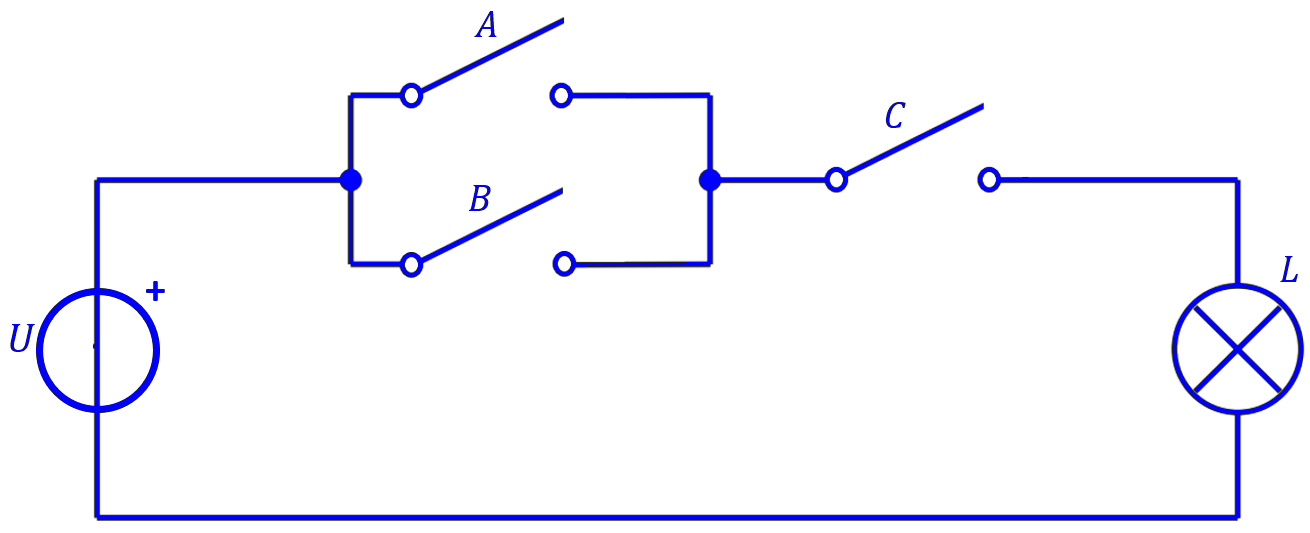
\includegraphics[width=\linewidth]{figurenAuteur/complexe_schakeling1.jpg}
\captionof{figure}{Combinatie van OR- en AND-schakeling}
\label{compl1}
\end{center}


\begin{center}
\begin{tabular}{c|c|c|c|c}  
$A$ & $B$ & $C$ & $A+B$ & $L=(A+B)\cdot C$ \\
   &     &      & $A\lor B$ & $(A\lor B)\land C$\\
\hline
1 & 1 & 1 & 1 & 1\\
1 & 1 & 0 & 1 & 0\\
1 & 0 & 1 & 1 & 1\\
1 & 0 & 0 & 1 & 0\\
0 & 1 & 1 & 1 & 1\\
0 & 1 & 0 & 1 & 0\\
0 & 0 & 1 & 0 & 0\\
0 & 0 & 0 & 0 & 0\\
\end{tabular}
\captionof{table}{}
\label{tabelORAND}
\end{center}

Bij het `rekenen' met de nieuwe som (OR) en het nieuwe product (AND) zoals we dat hierboven gedefinieerd hebben, kunnen we nagaan of de gekende regels van commutativiteit, associativiteit enz. nog gelden. We rekenen dan met deze schakelingen (of we kunnen dat ook doen in propositielogica) alsof we rekenen met getallen. We spreken in die context van boole-algebra of booleaanse algebra, vernoemd naar de uitvinder ervan, de Britse wiskundige en logicus George Boole (1815-1864). Lang voor er sprake was van computers werkte hij de algebra uit die nu nog steeds in elk computersysteem gebruikt wordt. Daarom wordt hij beschouwd als één van de grondleggers van de computerwetenschap.

In figuur \ref{compl2} zie je een andere schakeling. In dit schema komt de schakelaar $C$ twee
keer voor. Deze schakelaars zijn op één of andere manier gekoppeld zodat beide schakelaars steeds tegelijk van stand veranderen (en dezelfde logische waarde hebben in de waarheidstabel).

Met de notaties uit de propositielogica kun je deze schakeling noteren als $(A\land C) \lor (B\land C)$. De lamp brandt als schakelaars A en C óf B en C geactiveerd zijn.

\begin{center}
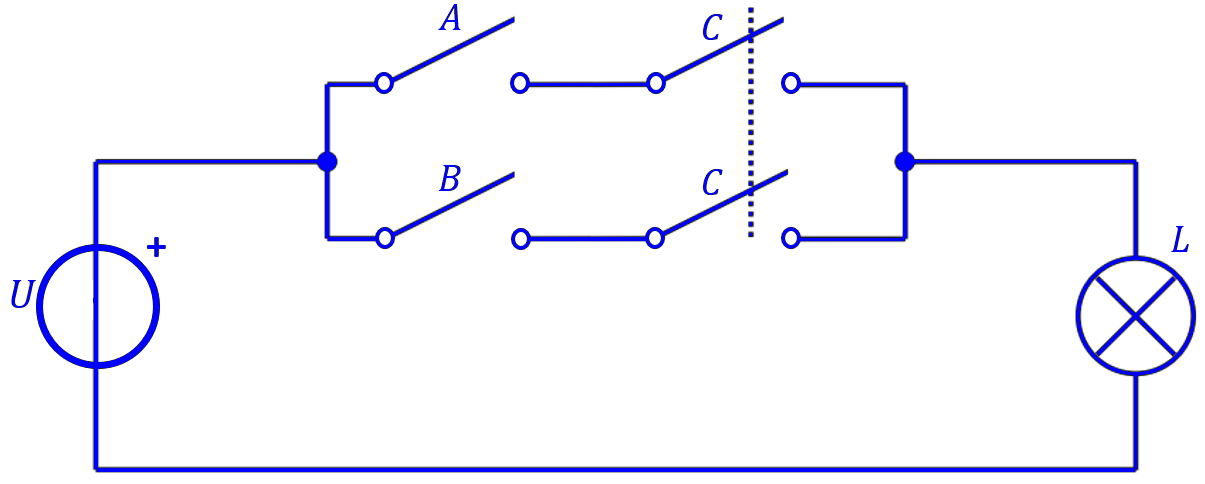
\includegraphics[width=\linewidth]{figurenAuteur/complexe_schakeling2.jpg}
\captionof{figure}{Combinatie van AND- en OR-schakelingen}
\label{compl2}
\end{center}

\begin{center}
\begin{tabular}{c|c|c|c|c|c}  
$A$ & $B$ & $C$ & $A\cdot C$ & $B\cdot C$ &  $L=(A\cdot C)+ (B\cdot C)$ \\
   &     &      & $A\land C$ & $B\land C$ & $(A\land C) \lor (B\land C)$\\
\hline
1 & 1 & 1 & 1 & 1 & 1\\
1 & 1 & 0 & 0 & 0 & 0\\
1 & 0 & 1 & 1 & 0 & 1\\
1 & 0 & 0 & 0 & 0 & 0\\
0 & 1 & 1 & 0 & 1 & 1\\
0 & 1 & 0 & 0 & 0 & 0\\
0 & 0 & 1 & 0 & 0 & 0 \\
0 & 0 & 0 & 0 & 0 & 0\\
\end{tabular}
\captionof{table}{}
\label{tabelANDOR}
\end{center}



Vergelijk tabel \ref{tabelORAND} met tabel \ref{tabelANDOR}: we stellen vast dat $$(A\lor B)\land C\Leftrightarrow (A\land C) \lor (B\land C)$$ een tautologie is. We noemen dit de distributiviteit van $\land$ t.o.v. $\lor$. Anders genoteerd: $$L=(A+B)\cdot C=A\cdot C +B\cdot C.$$  De twee schakelingen uit figuur \ref{compl1} en figuur \ref{compl2} hebben dus helemaal hetzelfde effect.


\subsection{Logische poorten}

We vermeldden hierboven al dat een processor van een computer bestaat uit digitale schakelingen. We werkten tot nu met kringen met schakelaars en een lamp. Je zou die schakelaars als een soort van ingang kunnen bekijken en de lamp als uitgang. Natuurlijk bevinden er zich in de processor van een computer geen duizenden lampjes. Vanaf het midden van de jaren `60 van de vorige eeuw gebruikt men voor die processor geïntegreerde schakelingen (integrated circuits, ic’s of chips) die zijn opgebouwd met enkele logische poorten. Een logische poort is een elektronische schakeling met één of meerdere ingangen en juist één uitgang (zie de pinnetjes uit figuur \ref{intfoto7408ic} of de cijfers in het schema bij figuur \ref{intpinout7408}). De logische toestand van de uitgang is $0$ of $1$, wat overeenkomt met spanningsniveau L(ow) of H(igh), zoals hierboven beschreven. Deze toestand wordt enkel en alleen bepaald door de logische toestand van de ingangen. De basispoorten zijn AND-, OR- en NOT-poorten. Deze worden gecombineerd om andere logische schakelingen te maken. De uitgang van de ene poort kun je gebruiken als ingang van een volgende poort.  Er zijn ontzettend veel ic's, elk met hun eigen functie en poortschakelingen. 

Een voorbeeld van zo'n chip zie je in figuur~\ref{intfoto7408ic}. Je ziet een blokje met aan weerszijden zeven aansluitpinnen. Met deze aansluitpinnen kun je in- en uitgangen van de 
poortschakelingen aansluiten. Het ic bevat binnenin vier AND-poorten met drie aansluitingen elk. Daarnaast zijn nog twee voedingsspanningsaansluitingen nodig zodat het totaal op veertien aansluitingen komt. 

\begin{center}
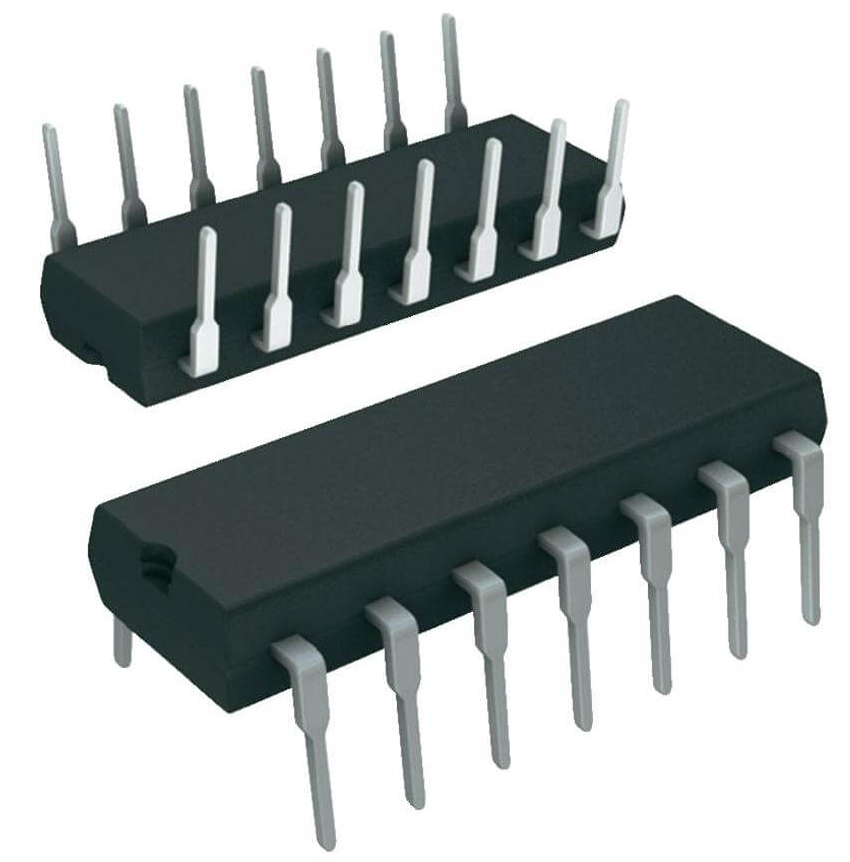
\includegraphics[width=0.5\linewidth]{figurenAuteur/intfoto7408ic_2.jpg}
\captionof{figure}{7408 Quad 2-input AND gate, een ic-poort}
\label{intfoto7408ic}
\end{center}

\begin{center}
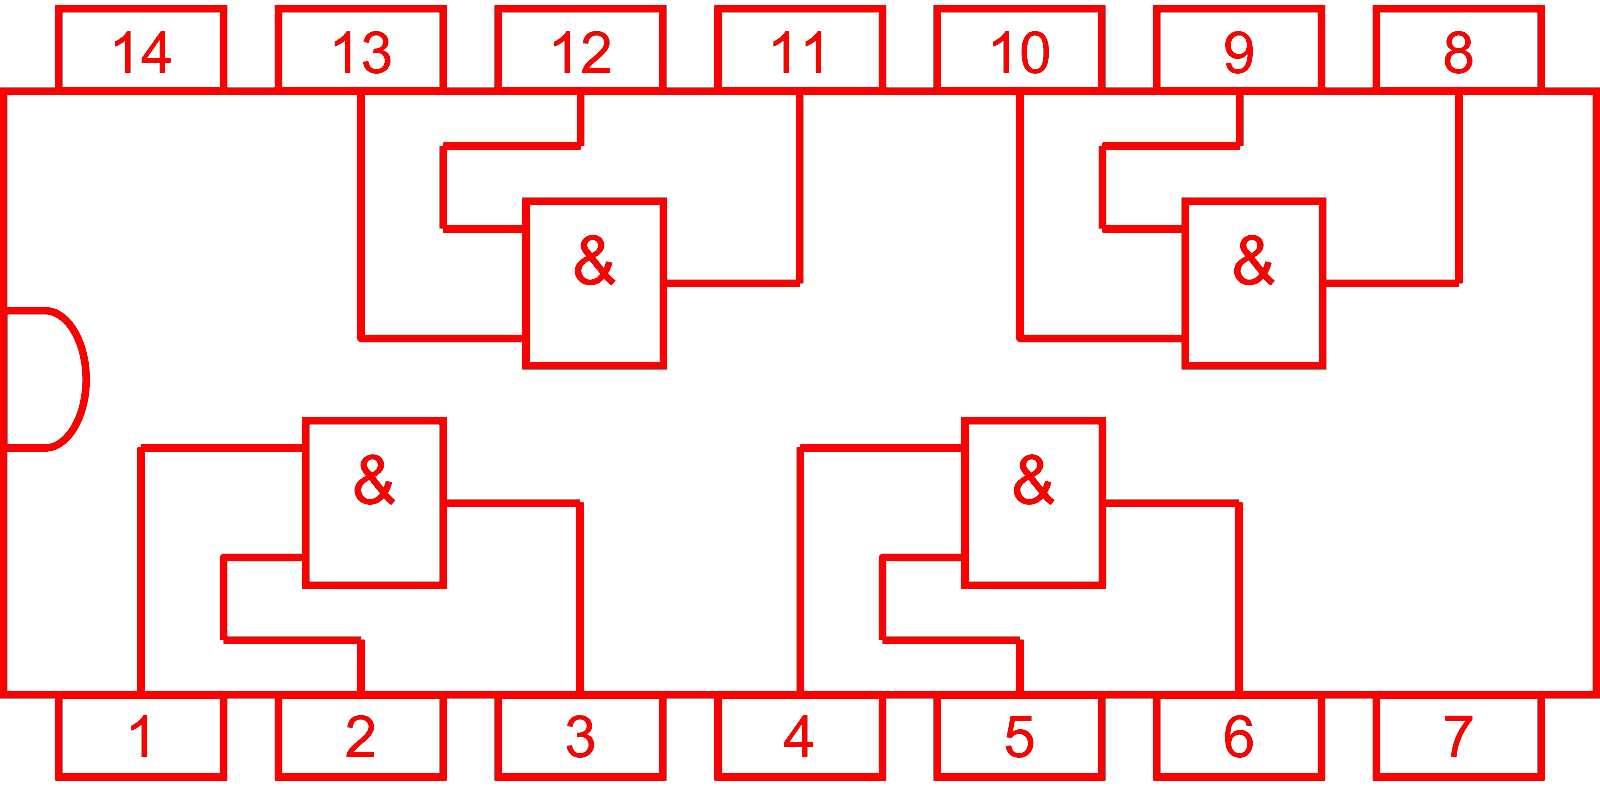
\includegraphics[width=0.8\linewidth]{figurenAuteur/intpinout7408.jpg}
\captionof{figure}{Vier AND-poorten met elk drie aansluitingen}
\label{intpinout7408}
\end{center}

Het schema van deze chip is te zien in figuur~\ref{intpinout7408}. De symbolen die hierin gebruikt worden, worden in de volgende paragraaf verklaard. 

We behandelen nu de belangrijkste logische poorten.

\tussentitel{AND-poort}
Een AND-poort is een schakeling met één uitgang en meerdere
ingangen, waarbij de uitgang slechts 1 is als en slechts als alle ingangen 1 zijn. De
uitgang wordt 0 van zodra minstens één ingang 0 wordt.

Uit de definitie kunnen we de volgende waarheidstabel afleiden (voor 2 ingangen
$A$ en $B$ en uitgang $Y$):

\begin{center}
\begin{tabular}{c|c|c}  
$A$ & $B$ & $Y=A\cdot B$\\
\hline
1 & 1 & 1 \\
1 & 0 & 0\\
0 & 1 & 0\\
0 & 0 & 0
\end{tabular}
\captionof{table}{Waarheidstabel bij de AND-poort}
\end{center}

We herkennen de conjunctie en zien dat $Y$ logisch equivalent is met $A\land B$. De AND-poort doet eigenlijk hetzelfde als de logische schakeling in figuur \ref{serie}. De schematische voorstelling is echter veel compacter, zie figuur \ref{and-poort}. Het aantal ingangen kan uitgebreid worden, maar het minimum is twee.

\begin{center}
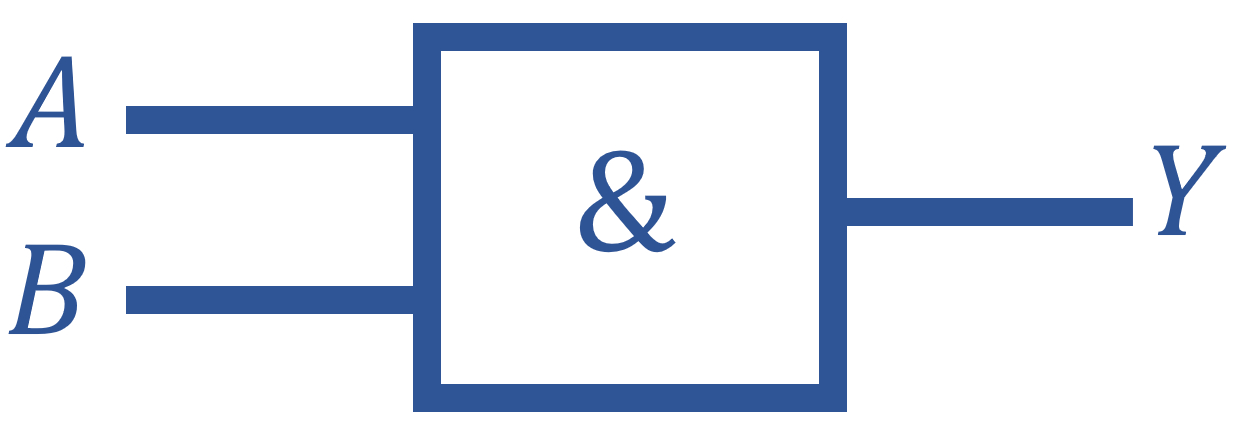
\includegraphics[width=0.45\linewidth]{figurenAuteur/intsymboolandieee_eigen1.jpg}
\hspace{0.05\linewidth}
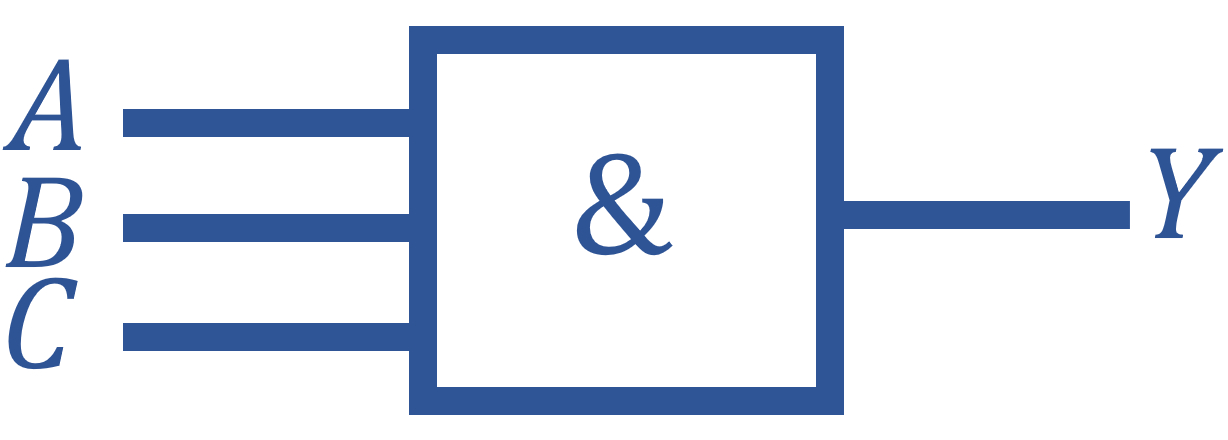
\includegraphics[width=0.45\linewidth]{figurenAuteur/intsymboolandieee_eigen2.jpg}
\captionof{figure}{Symbolische voorstelling van de AND-poort, zowel met twee als met drie ingangen}
\label{and-poort}
\end{center}

Je kunt gemakkelijk aantonen (waarheidstabel) dat $A\land B$ logisch equivalent is met $B\land A$. De volgorde van de ingangen speelt dus geen rol.



\tussentitel{OR-poort}

Een OR-poort is een schakeling met één uitgang en meerdere
ingangen, waarbij de uitgang 1 is van zodra minstens één ingang 1 is. De
uitgang wordt 0 als en slechts als alle ingangen 0 zijn.

Uit de definitie kunnen we de volgende waarheidstabel afleiden (voor 2 ingangen
$A$ en $B$ en uitgang $Y$):

\begin{center}
\begin{tabular}{c|c|c}  
$A$ & $B$ & $Y=A+B$\\
\hline
1 & 1 & 1 \\
1 & 0 & 1\\
0 & 1 & 1\\
0 & 0 & 0
\end{tabular}
\captionof{table}{Waarheidstabel bij de OR-poort}
\end{center}

We herkennen de disjunctie en zien dat $Y$ logisch equivalent is met $A\lor B$. De OR-poort doet eigenlijk hetzelfde als de logische schakeling in figuur \ref{parallel}. De schematische voorstelling is opnieuw veel compacter, zie figuur \ref{or-poort}. Het aantal ingangen kan uitgebreid worden, maar het minimum is twee.

\begin{center}
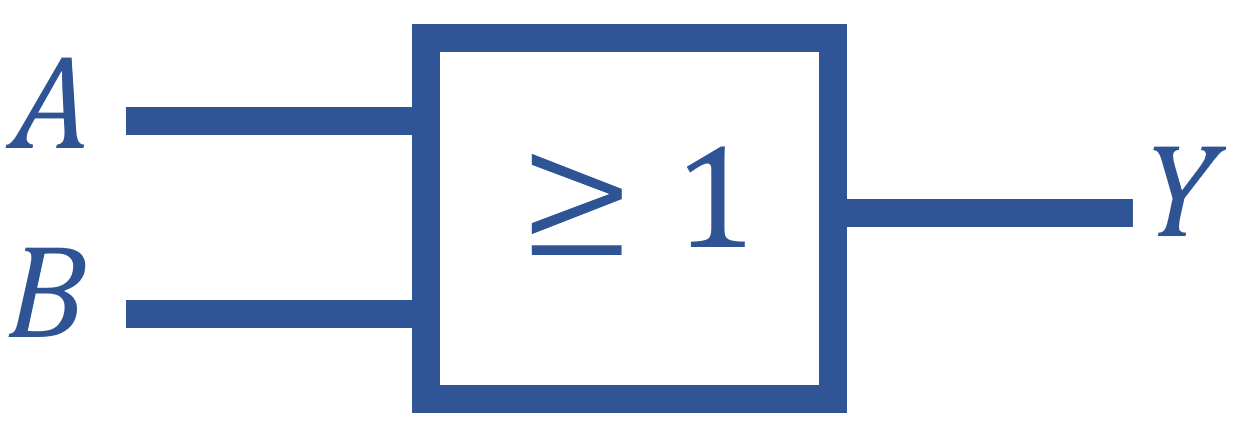
\includegraphics[width=0.45\linewidth]{figurenAuteur/intsymboolorieee_eigen1.jpg}
\hspace{0.05\linewidth}
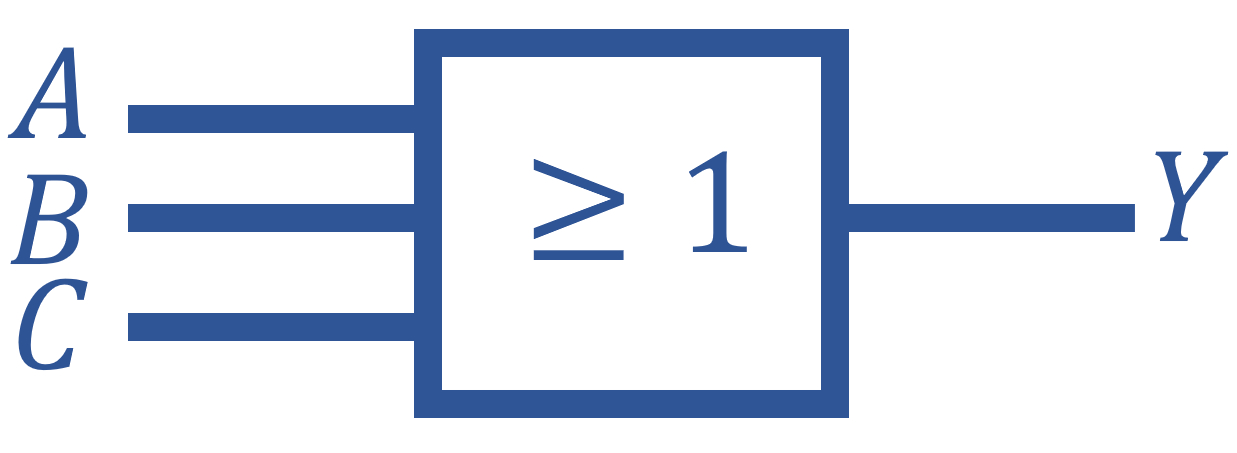
\includegraphics[width=0.45\linewidth]{figurenAuteur/intsymboolorieee_eigen2.jpg}
\captionof{figure}{Symbolische voorstelling van de OR-poort, zowel met twee als met drie ingangen}
\label{or-poort}
\end{center}

Merk op dat de aanduiding $\geq 1$ in de symbolische voorstelling van de OR-poort heel logisch is: als de som van de waarden van de ingangen $A$, $B$$\ldots$ minstens $1$ is, dan is de logische waarde van de uitgang $Y$ ook 1.


Je kunt gemakkelijk aantonen (waarheidstabel) dat $A\lor B$ logisch equivalent is met $B\lor A$. De volgorde van de ingangen speelt dus geen rol.



\tussentitel{NOT-poort}

Een NOT-poort of invertor is een schakeling met één ingang en één uitgang,
waarbij de uitgang altijd de inverse toestand heeft van de ingang. De uitgang is
dus $1$ als de ingang $0$ is en de uitgang is $0$ als de ingang $1$ is.

Uit de definitie kunnen we de volgende waarheidstabel afleiden (voor ingang
$A$ en uitgang $Y$):

\begin{center}
\begin{tabular}{c|c}  
$A$ & $Y$\\
\hline
1 & 0\\
0 & 1
\end{tabular}
\captionof{table}{Waarheidstabel bij de NOT-poort}
\end{center}

We herkennen de negatie en zien dat $Y$ logisch equivalent is met $\lnot A$. De NOT-poort doet eigenlijk hetzelfde als de logische schakeling in figuur \ref{not}. De schematische voorstelling zie je in figuur \ref{not-poort}.

\begin{center}
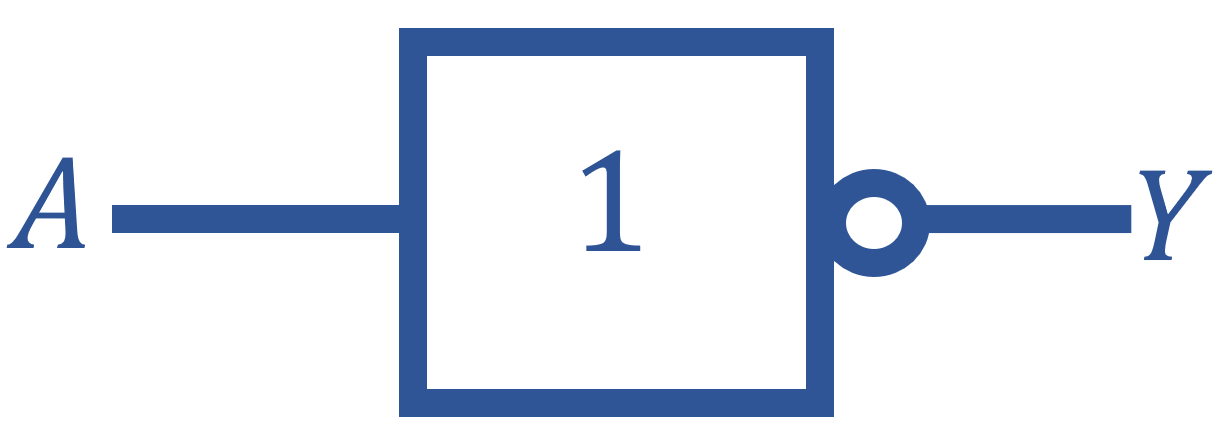
\includegraphics[width=0.45\linewidth]{figurenAuteur/intsymboolnotieee_eigen.jpg}
\captionof{figure}{Symbolische voorstelling van de NOT-poort}
\label{not-poort}
\end{center}

Met de logische poorten AND, OR en NOT kunnen we elke logische schakeling, hoe ingewikkeld ook, volledig opbouwen. In de volgende oefening bekijken we een iets complexere schakeling.

\end{multicols}

\beginwerktekst{Een logische schakeling opgebouwd met poorten}

Bekijk de volgende schakeling met poorten:
\begin{center}
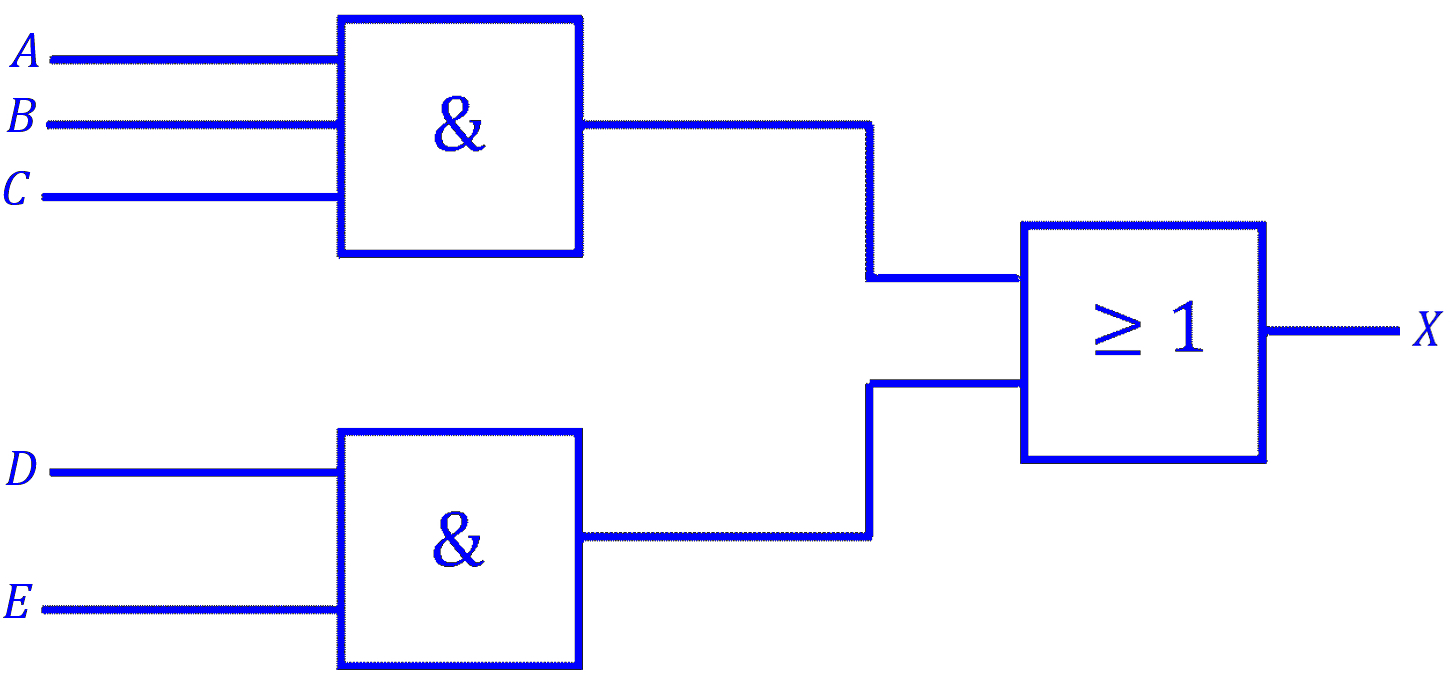
\includegraphics[width=0.55\linewidth]{figurenAuteur/schakeling1.jpg}
\end{center}

\begin{werktekstoef}

\item{Met welke propositie is $X$ logisch equivalent?}

\emph{$X$ is logisch equivalent met $(A\land B\land C)\lor (D\land E)$}

\item{Geef de logische vergelijking die bij deze schakeling hoort.}

\emph{$X=A\cdot B\cdot C + D\cdot E$}

\item{Hoeveel lijnen heeft de waarheidstabel van deze schakeling?}

\emph{Er zijn 5 ingangen, dus is het aantal lijnen gelijk aan $2^5=32$.}

\item{Als $A$, $D$ en $E$ logische toestand $1$ hebben en $B$ en $C$ hebben toestand $0$, bepaal dan de logische toestand van $X$.}

\emph{De logische waarde van $A\land B\land C$ is dan $0$ en die van $D\land E$ is $1$. Bijgevolg is de waarde van  $(A\land B\land C)\lor (D\land E)$ gelijk aan 1.}

\end{werktekstoef}  
\eindewerktekst


\begin{multicols}{2}

Om het eenvoudiger te maken, heeft men ook afgeleide poorten ingevoerd. Hieronder volgen enkele voorbeelden.

%\vspace{10mm}

\tussentitel{NAND-poort}
Een NAND-poort is een AND-poort gevolgd door een NOT-poort, zoals in figuur \ref{nand-poort}.

Het is een mooie oefening om uit deze definitie de waarheidstabel af te leiden (voor 2 ingangen $A$ en $B$ en uitgang $Y$):

\begin{center}
\begin{tabular}{c|c|c}  
$A$ & $B$ & $Y=\overline{A\cdot B}$\\
\hline
1 & 1 & 0 \\
1 & 0 & 1\\
0 & 1 & 1\\
0 & 0 & 1
\end{tabular}
\captionof{table}{Waarheidstabel bij de NAND-poort}
\end{center}

We zien dat $Y$ logisch equivalent is met $\lnot(A\land B)$.\\
De NAND-poort is een schakeling waarin de uitgang $1$ wordt van zodra één of meerdere ingangen
$0$ zijn. De uitgang kan enkel $0$ zijn als en slechts als alle ingangen $1$ zijn.


\begin{center}
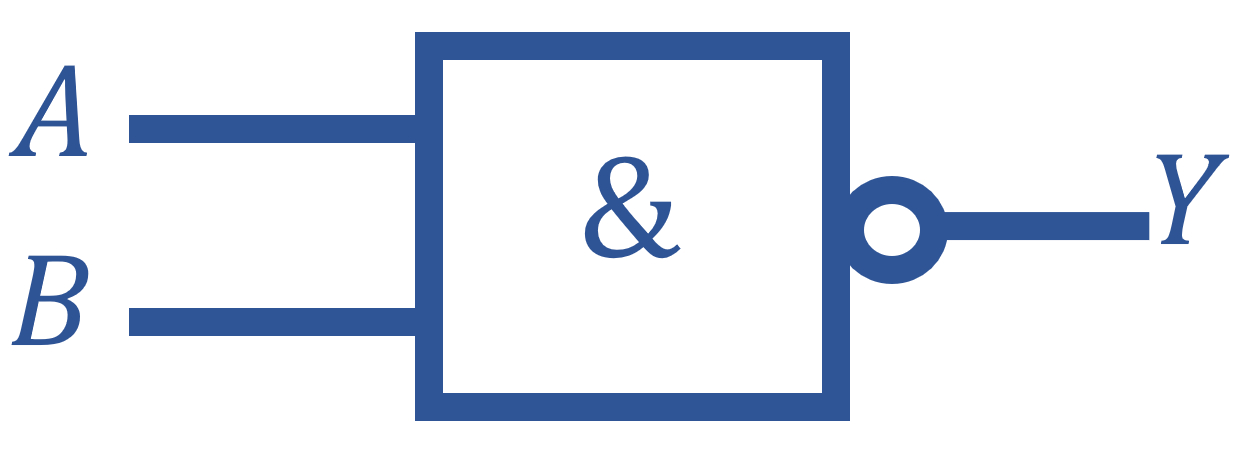
\includegraphics[width=0.45\linewidth]{figurenAuteur/intsymboolnandieee_eigen1.jpg}
%\hspace{0.1\linewidth}
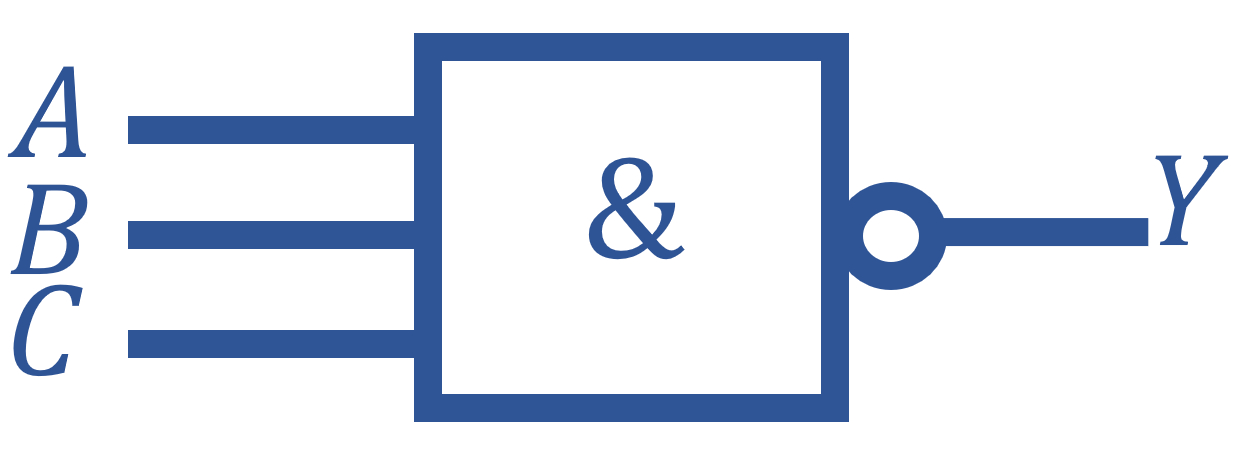
\includegraphics[width=0.45\linewidth]{figurenAuteur/intsymboolnandieee_eigen2.jpg}
\captionof{figure}{Symbolische voorstelling van de NAND-poort, zowel met twee als met drie ingangen}
\label{nand-poort}
\end{center}

Als oefening kun je de leerlingen de waarheidstabel laten maken van de NAND-poort met drie ingangen.

\tussentitel{NOR-poort}
Een NOR-poort is een OR-poort gevolgd door een NOT-poort, zoals in figuur \ref{nor-poort}.

Het is een mooie oefening om uit deze definitie de waarheidstabel af te leiden (voor 2 ingangen $A$ en $B$ en uitgang $Y$):

\begin{center}
\begin{tabular}{c|c|c}  
$A$ & $B$ & $Y=\overline{A+B}$\\
\hline
1 & 1 & 0 \\
1 & 0 & 0\\
0 & 1 & 0\\
0 & 0 & 1
\end{tabular}
\captionof{table}{Waarheidstabel bij de NOR-poort}
\end{center}

We zien dat $Y$ logisch equivalent is met $\lnot(A\lor B)$.\\
De NOR-poort is een schakeling waarbij de uitgang $0$ wordt van zodra één of meerdere ingangen
$1$ zijn. De uitgang kan enkel $1$ zijn als en slechts als alle ingangen $0$ zijn. Dit komt overeen met de Engelse uitdrukking `Neither $\ldots$ nor $\ldots$' 

Als oefening kun je de leerlingen de waarheidstabel laten maken van de NOR-poort met drie ingangen.


\begin{center}
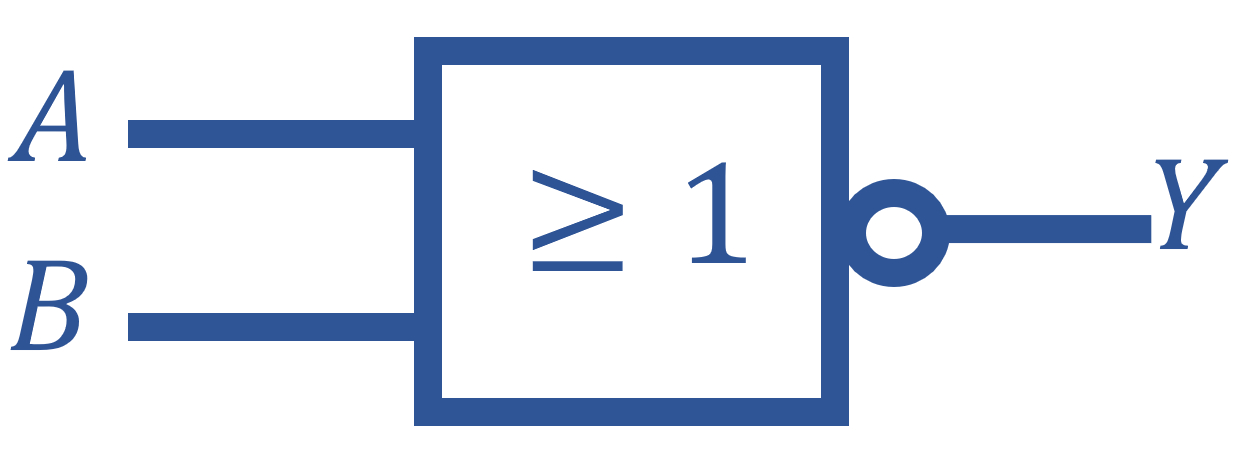
\includegraphics[width=0.45\linewidth]{figurenAuteur/intsymboolnorieee_eigen1.jpg}
%\hspace{0.1\linewidth}
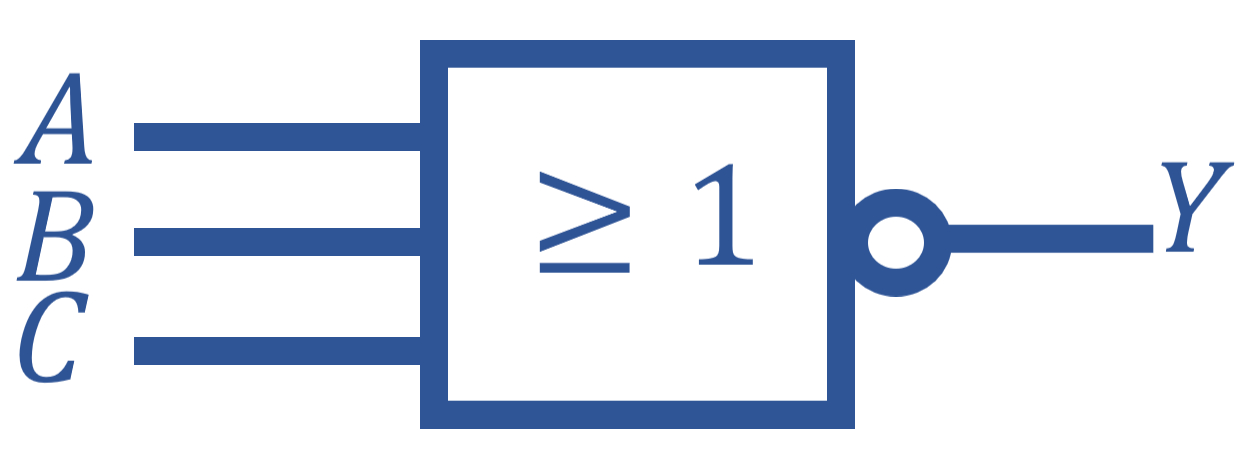
\includegraphics[width=0.45\linewidth]{figurenAuteur/intsymboolnorieee_eigen2.jpg}
\captionof{figure}{Symbolische voorstelling van de NOR-poort, zowel met twee als met drie ingangen}
\label{nor-poort}
\end{center}


\tussentitel{XOR-poort}

We vermeldden hierboven al dat de `of' in propositielogica een inclusieve of is. De OR-poort van hierboven is ook een inclusieve of. We kunnen de exclusieve of maken m.b.v. logische poorten en we spreken dan van de XOR-poort.

De uitgang van een XOR-poort wordt 1 als juist één van de ingangen
1 is, anders wordt de uitgang 0. Anders gezegd: de uitgang wordt
1 als de ingangen niet gelijk zijn aan elkaar, anders wordt de uitgang 0.

De waarheidstabel voor 2 ingangen $A$ en $B$ en uitgang $Y$:

\begin{center}
\begin{tabular}{c|c|c}  
$A$ & $B$ & $Y$\\
\hline
1 & 1 & 0 \\
1 & 0 & 1\\
0 & 1 & 1\\
0 & 0 & 0
\end{tabular}
\captionof{table}{Waarheidstabel bij de XOR-poort}
\end{center}

\begin{center}
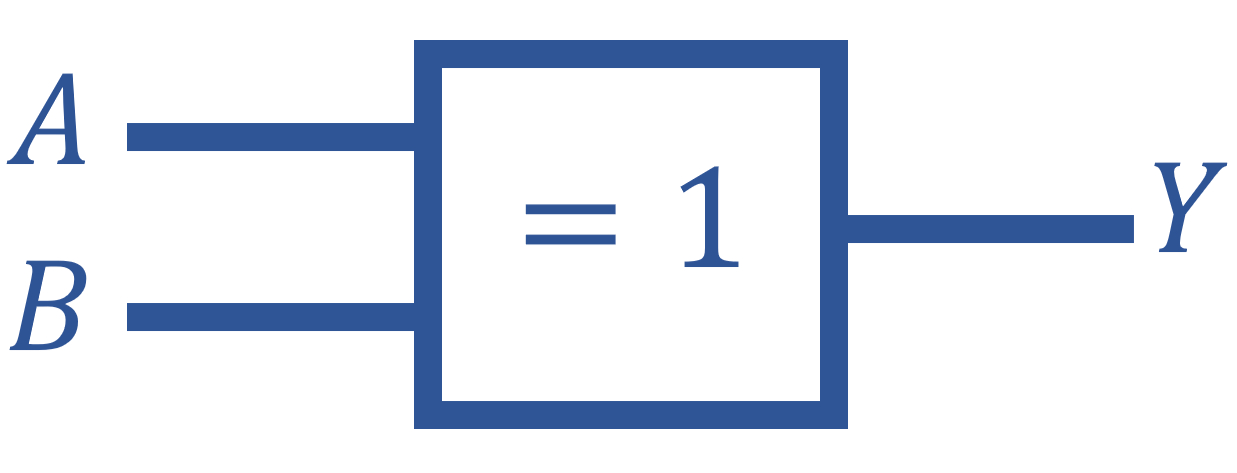
\includegraphics[width=0.45\linewidth]{figurenAuteur/intsymboolxorieee_eigen.jpg}
\captionof{figure}{Symbolische voorstelling van de XOR-poort}
\label{xor-poort}
\end{center}

Merk op dat de aanduiding $=1$ in de symbolische voorstelling van de XOR-poort niet toevallig is gekozen: als de (gewone) som van de waarden van de ingangen $A$ en $B$ exact $1$ is dan is de logische waarde van de uitgang $Y$ ook 1.

Je kunt narekenen (waarheidstabel): $$Y=A\cdot \overline{B}+\overline{A}\cdot B$$ of ook $$Y=(A+B)\cdot (\overline{A}+\overline{B}).$$ Men noteert dit verkort ook als $$Y=A\oplus B.$$
Verderop zullen we een schakeling tegenkomen die equivalent is met de XOR-poort en die enkel NAND-poorten bevat.


\tussentitel{Amerikaanse symbolen}

Wij gebruikten hierboven de Britse IEC-symbolen (International Electrotechnical Commission) voor de verschillende logische poorten. Heel vaak worden ook de Amerikaanse ANSI-vormsymbolen gebruikt (American National Standard of Industry). Er is ook nog een Duits DIN-systeem (Deutsche Institut für Normung). In figuur \ref{vorm} zie je een overzicht van de Amerikaanse vormsymbolen. Het is niet de bedoeling dat leerlingen verschillende systemen leren. We vermelden dit voor collega's die Amerikaanse opgaven vinden en ze in de klas willen gebruiken. Ze kunnen die dan eenvoudig aanpassen aan het Britse systeem.

\begin{center}
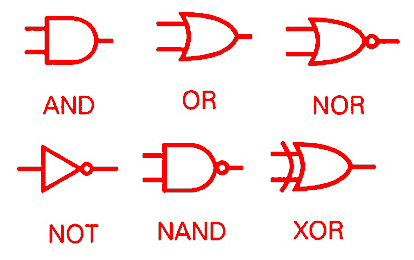
\includegraphics[width=\linewidth]{figurenAuteur/vorm.jpg}
\captionof{figure}{Overzicht van de veel gebruikte Amerikaanse vormsymbolen voor logische poorten}
\label{vorm}
\end{center}

In de volgende lesactiviteit maken we oefeningen waarbij de leerlingen o.a. moeten wisselen tussen de voorstellingen van een schakeling. Uit het schema moeten ze een waarheidstabel afleiden, de logische vergelijking afleiden en dit zowel noteren met de notaties uit propositielogica als die uit boole-algebra. De tabel of de logische vergelijking kan worden gebruikt om equivalente schakelingen te zoeken of om schakelingen te vereenvoudigen.


\end{multicols}


\beginwerktekst{Schakelingen en logische poorten}

\begin{nummering}
\item Gegeven is de volgende schakeling met poorten:
\begin{center}
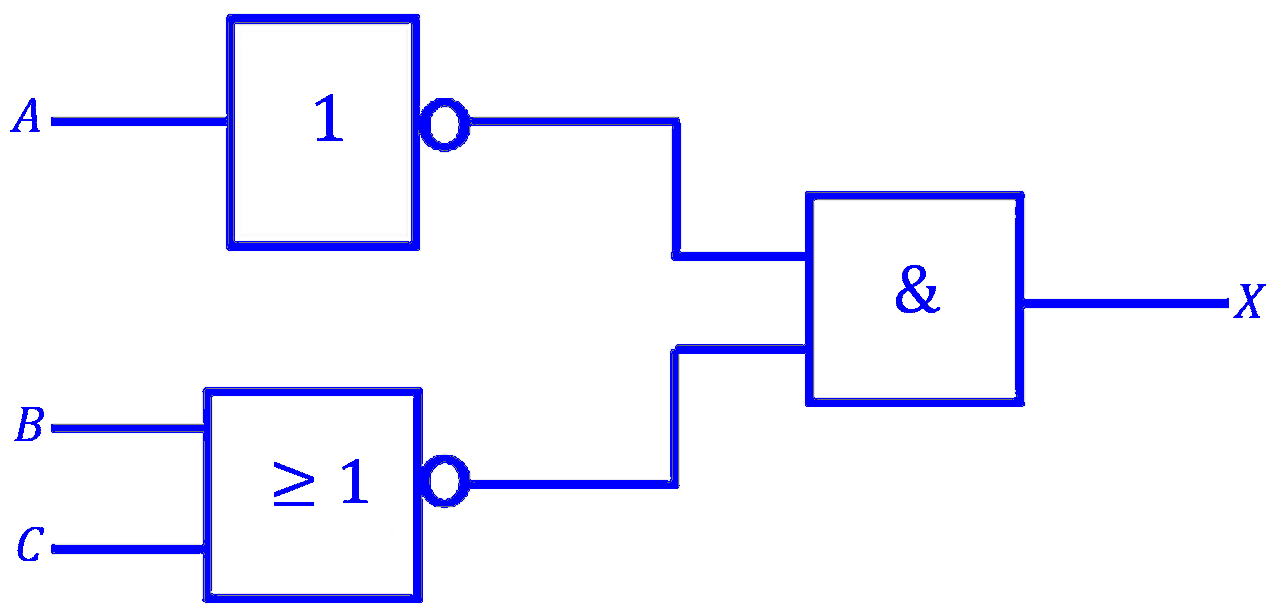
\includegraphics[width=0.45\linewidth]{figurenAuteur/schakeling3.jpg}
\end{center}
    
\begin{werktekstoef}
\item[a.]{Welke propositie hoort bij $X$? Geef ook de logische vergelijking.}

\emph{$X$ is logisch equivalent met $\lnot A \land \lnot(B\lor C)$. De logische vergelijking is $X=\overline{A}\cdot \overline{B+C}$. Met waarheidstabellen kun je aantonen dat dit laatste ook gelijk is aan $\overline{A}\cdot \overline{B}\cdot \overline{C}$.}

\item[b.]{Stel de waarheidstabel op die bij deze schakeling hoort.}

\emph{De waarheidstabel bij deze schakeling:}
\begin{center}
\begin{tabular}{c|c|c|c|c|c|c}  
$A$ & $B$ & $C$ & $\overline{A}$ & $B+C$ & $\overline{B+C}$ & $X=\overline{A}\cdot \overline{B+C}$ \\
   &     &      & $\lnot A$ & $B\lor C$ & $\lnot (B\lor C)$ & $\lnot A \land \lnot(B\lor C)$\\
\hline
1 & 1 & 1 & 0 & 1 & 0 & 0\\
1 & 1 & 0 & 0 & 1 & 0 & 0\\
1 & 0 & 1 & 0 & 1 & 0 & 0\\
1 & 0 & 0 & 0 & 0 & 1 & 0\\
0 & 1 & 1 & 1 & 1 & 0 & 0\\
0 & 1 & 0 & 1 & 1 & 0 & 0\\
0 & 0 & 1 & 1 & 1 & 0 & 0\\
0 & 0 & 0 & 1 & 0 & 1 & 1\\
\end{tabular}
\end{center}

\end{werktekstoef}


\item Gegeven is de volgende schakeling met poorten:
\begin{center}
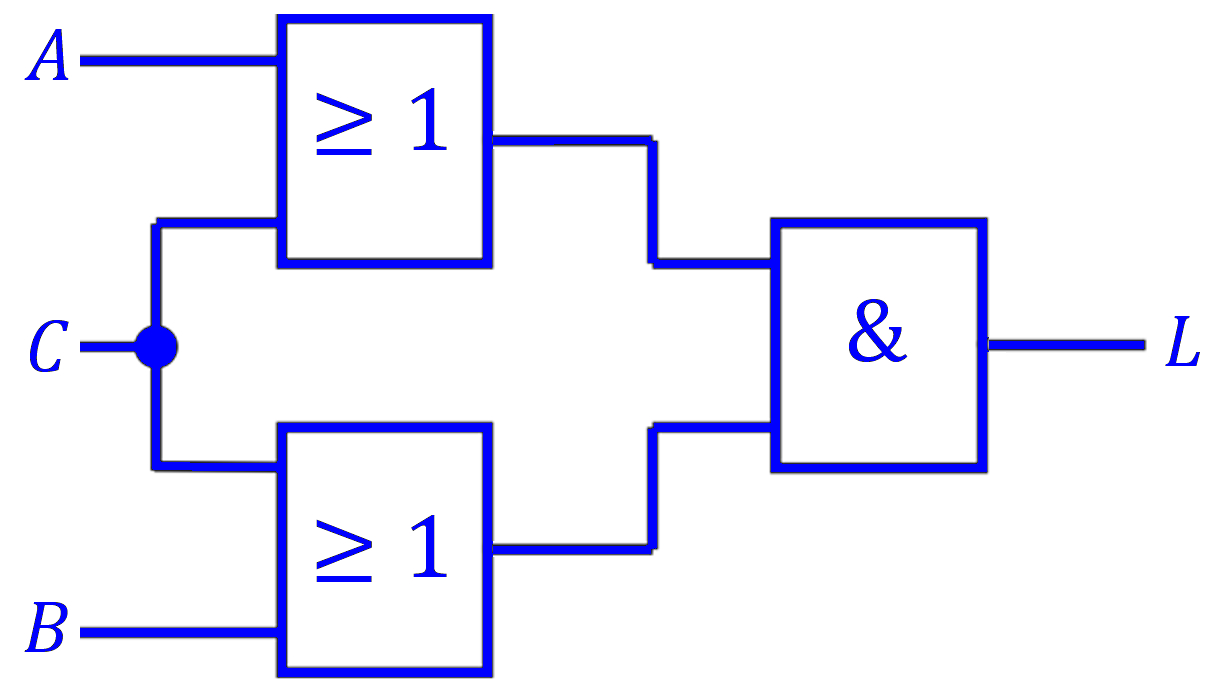
\includegraphics[width=0.4\linewidth]{figurenAuteur/schakeling2.jpg}
\end{center}

\begin{werktekstoef}
\item[a.]{Met welke propositie is $L$ logisch equivalent? Geef ook de logische vergelijking.}

\emph{$L$ is logisch equivalent met $(A\lor C)\land (B\lor C)$. De logische vergelijking is $L=(A+ C) \cdot (B+ C)$.}

\item[b.]{Maak een waarheidstabel die hoort bij deze schakeling. Hiermee kun je inschatten wat die schakeling doet.}

\emph{De waarheidstabel bij deze schakeling:}
\begin{center}
\begin{tabular}{c|c|c|c|c|c}  
$A$ & $B$ & $C$ & $A+C$ & $B+C$  & $L=(A+ C) \cdot (B+ C)$ \\
   &     &      & $A\lor C$ & $B\lor C$ & $(A\lor C)\land (B\lor C)$\\
\hline
1 & 1 & 1 & 1 & 1 & 1 \\
1 & 1 & 0 & 1 & 1 & 1 \\
1 & 0 & 1 & 1 & 1 & 1 \\
1 & 0 & 0 & 1 & 0 & 0 \\
0 & 1 & 1 & 1 & 1 & 1 \\
0 & 1 & 0 & 0 & 1 & 0 \\
0 & 0 & 1 & 1 & 1 & 1 \\
0 & 0 & 0 & 0 & 0 & 0 \\
\end{tabular}
\end{center}


\item[c.]{Zoek een andere schakeling die hetzelfde effect heeft. Teken deze schakeling ook.}

\emph{De vergelijking $L=(A+ C) \cdot (B+ C)$ is te herschrijven tot $L=(A\cdot B)+ C$. Je kunt dit zien als een soort van distributieve eigenschap. Om die te bewijzen kun je de waarheidstabellen vergelijken. Daaruit blijkt dat inderdaad: $L=(A+ C) \cdot (B+ C)=(A\cdot B)+ C$. Anders gezegd: de uitspraak $(A\lor C) \land (B\lor C) \Leftrightarrow (A\land B)\lor C$ is een tautologie. Dit komt overeen met volgende schakeling:}

\begin{center}
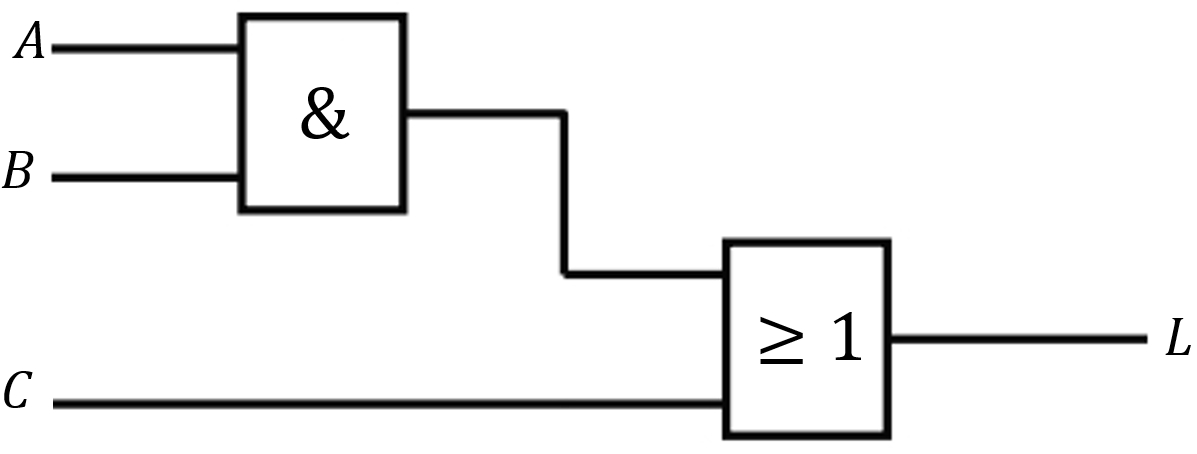
\includegraphics[width=0.45\linewidth]{figurenAuteur/schakeling2_opl.jpg}
\end{center}

\emph{Dit is een vereenvoudiging van de oorspronkelijke schakeling.}


\end{werktekstoef}


\item Bekijk de volgende schakeling die enkel NAND-poorten bevat:
\begin{center}
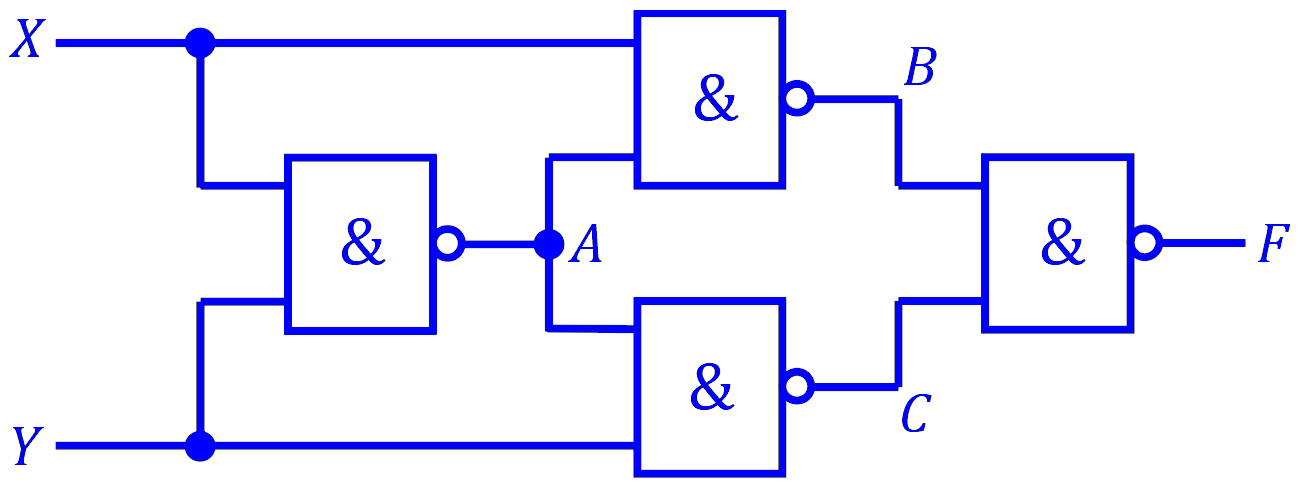
\includegraphics[width=0.45\linewidth]{figurenAuteur/intxor4nands.jpg}
\end{center}

\begin{werktekstoef}


\item[a.]{Maak een waarheidstabel voor deze schakeling}

\emph{Bepaal de waarde bij elke (tussen)uitgang:}
\begin{center}
\begin{tabular}{c c|c c c|c}  
$X$ & $Y$ & $A$ & $B$ & $C$ & $F$\\
\hline
0 & 0 & 1 & 1 & 1 & 0 \\
0 & 1 & 1 & 1 & 0 & 1 \\
1 & 0 & 1 & 0 & 1 & 1 \\
1 & 1 & 0 & 1 & 1 & 0 
\end{tabular}
\end{center}

\item[b.]{Wat stel je vast?}

\emph{Deze schakeling heeft hetzelfde effect als de XOR-poort.}

\item[c.]{Toon aan: $\overline{U\cdot V}=\overline{U}+\overline{V}$.}

\emph{Dit kun je doen door de waarheidstabel te maken van $\overline{U\cdot V}$ en deze te vergelijken met die van $\overline{U}+\overline{V}$.}

\item[d.]{Bepaal de logische vergelijking bij de schakeling uit de figuur. Gebruik hierbij de eigenschap uit (c).}

\emph{Dit is niet zo gemakkelijk en zal voor de meeste leerlingen veel begeleiding vragen. Het illustreert wel mooi hoe rekenen in boole-algebra verloopt.
\begin{align*}
F&=\overline{B\cdot C}\\
&=\overline{B}+\overline{C}\\
&=\overline{\overline{X\cdot A}} + \overline{\overline{Y\cdot A}}\\
&= X\cdot A +Y\cdot A \\
&= X\cdot \overline{X\cdot Y}+ Y\cdot \overline{X\cdot Y}\\
&= X\cdot (\overline{X}+\overline{Y})+Y\cdot (\overline{X}+\overline{Y})\\
\end{align*}
Je kunt met waarheidstabellen aantonen dat het laatste ook gelijk is aan $F=(X+Y)\cdot (\overline{X}+\overline{Y})$.
}


\end{werktekstoef}  


\item Gegeven is de volgende schakeling. Hierbij staat $\lnot A$ voor een normally closed schakelaar.

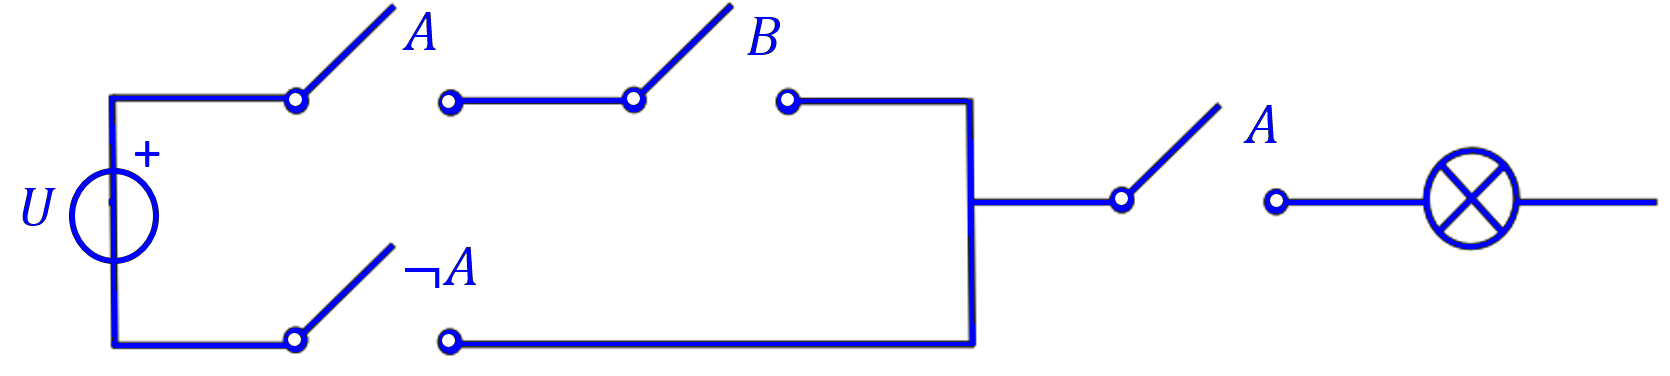
\includegraphics[width=0.6\linewidth]{figurenAuteur/schakeling6.jpg}
\begin{werktekstoef}
\item[a.] Teken deze schakeling met behulp van logische poorten.

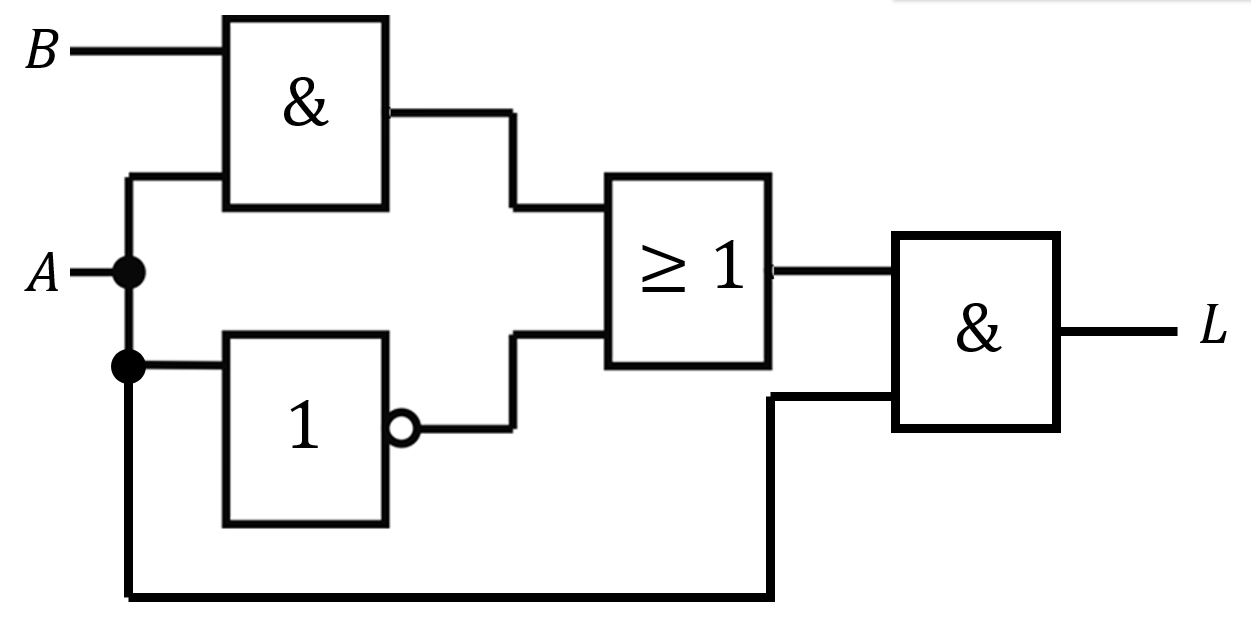
\includegraphics[width=0.4\linewidth]{figurenAuteur/schakeling6_opl.jpg}


\item[b.] Geef de logische vergelijking die bij deze schakeling hoort.

\emph{$L=\left( A\cdot B+\overline{A}\right)\cdot A$ of nog $\displaystyle \left((A\land B)\lor (\lnot A)\right)\land A$}

\item[c.] Vereenvoudig deze schakeling en teken ook de vereenvoudigde schakeling.

\emph{De waarheidstabel van de schakeling is}

\begin{center}
\begin{tabular}{c|c|c|c|c|c}  
$A$ & $B$ & $A\cdot B$ & $\overline A$ & $A\cdot B+\overline{A}$ & $L=\left( A\cdot B+\overline{A}\right)\cdot A$\\
    &     & $A\land B$ & $\lnot A$ & $(A\land B)\lor (\lnot A)$ & $\displaystyle \left((A\land B)\lor (\lnot A)\right)\land A$\\    
\hline
0 & 0 & 0 & 1 & 1 & 0 \\
0 & 1 & 0 & 1 & 1 & 0 \\
1 & 0 & 0 & 0 & 0 & 0 \\
1 & 1 & 1 & 0 & 1 & 1 
\end{tabular}
\end{center}

\emph{De lamp brandt dus enkel en alleen als schakelaar $A$ en schakelaar $B$ tegelijk gesloten zijn. Dit is een gewone AND-schakeling. Met de waarheidstabel hebben we nu bewezen dat
$\displaystyle  \left((A\land B)\lor (\lnot A)\right)\land A \Leftrightarrow A\land B$ een tautologie is of nog $L=\left( A\cdot B+\overline{A}\right)\cdot A=A\cdot B$.\\
De schakeling ziet er dus uit zoals in figuur \ref{serie}}.
%\begin{center}
%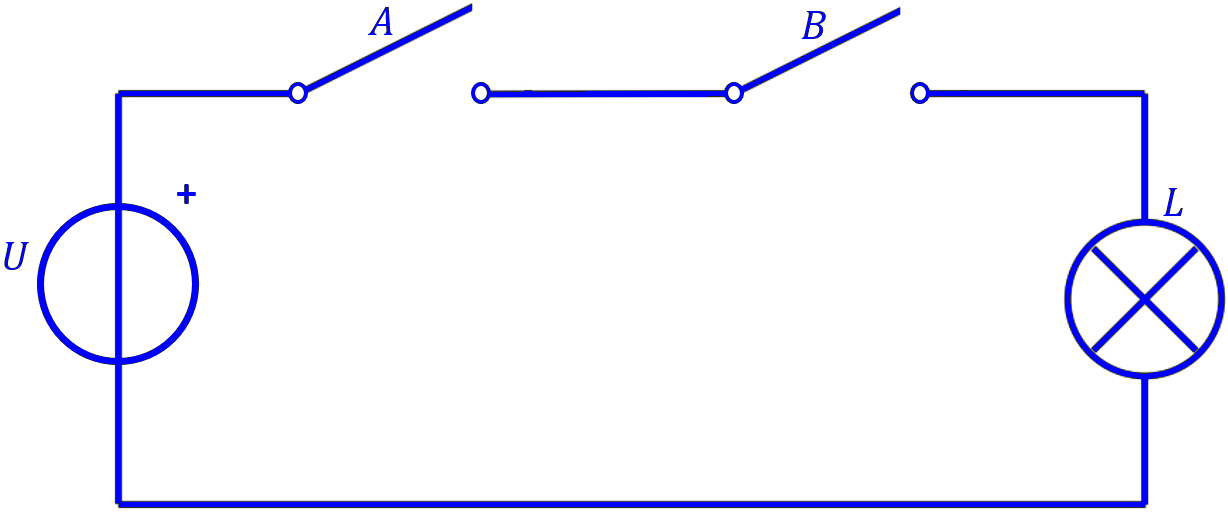
\includegraphics[width=0.3\linewidth]{figurenAuteur/serieschakeling.jpg}    
%\end{center}

\end{werktekstoef}

\end{nummering}
\eindewerktekst


\begin{multicols}{2}

\section{Beter zoeken met zoekmachines}
Op een fractie van een seconde doorzoekt een zoekmachine zoals Google 130 triljoen webpagina's aan de hand van jouw zoektermen. Je doet er vermoedelijk veel langer over om te gaan grasduinen in de resultaten. Maar wist je dat je veel gerichter naar informatie kunt zoeken door propositielogica te gebruiken? Het is naast een mooie oefening op de connectieven, een zeer relevante toepassing van logica in het dagelijks leven als je meerdere zoektermen tegelijkertijd hebt. We illustreren het aan de hand van Google.

\tussentitel{Zoeken naar exacte termen of een exacte woordengroep}
Dit eerste stukje heeft nog niets met logica te maken, maar is wel essentieel om Babylonische spraakverwarring te vermijden. Google is namelijk een erg geavanceerde zoekmachine geworden die bij het ingeven van een zoekterm als \verb|filmtips| niet per se naar die exacte term op zoek gaat, maar naar de meest relevante zoekresultaten die mogelijk verband houden met de ingegeven zoekterm. Zo vonden wij bij het ingeven van \verb|filmtips| meteen webpagina's die het woord filmtips niet exact bevatten, maar er wel mee verband hielden: `De vijftig beste films op Netflix', `11 ideeën voor een filmavond', `5 films voor een sprookachtige Halloween'... zijn enkele voorbeelden van topresultaten zonder dat ze expliciet het woord \verb|filmtips| bevatten. Wil je dat Google enkel zoekresultaten opneemt die letterlijk \verb|filmtips| bevatten? Plaats er dan dubbele aanhalingstekens rond: de zoekterm \verb|"filmtips"| zal uitsluitend pagina's retourneren die het woord filmtips letterlijk bevatten. Dat merk je ook als je het aantal geschatte zoekresultaten vergelijkt:

\begin{opsomming}
	\item zoekterm \verb|filmtips|: 943 000 resultaten,
	\item zoekterm \verb|"filmtips"|: 846 000 resultaten.
\end{opsomming}

Hetzelfde geldt voor woordengroepen: ben je op zoek naar filmtips met Tom Hanks? Dan zoek je best op \verb|filmtips "tom hanks"|. Google zal dan uitsluitend pagina's retourneren die exact Tom Hanks bevatten, de zoekterm \verb|filmtips tom hanks| laat ruimte om ook bv. films van Tom Cruise mee te krijgen in de resultaten. Zeker voor zeer concrete zoekopdrachten, waarbij je op zoek bent naar een specifieke combinatie van woorden (bv. de naam van een onbekend iemand die naamgelijkt op die van een bekend iemand), kun je met de dubbele aanhalingstekens veel gerichter zoeken en irrelevante, maar populaire, suggesties uitsluiten. Merk ook op dat de plaats van de dubbele aanhalingstekens uitmaakt: \verb|filmtips "tom hanks"| zoekt op pagina's die films suggereren met Tom Hanks, \verb|"filmtips tom hanks"| zoekt op pagina's die exact deze drie woorden na elkaar bevaten. Ook zijn de zoekopdrachten \verb|"Tom Hanks"| en \verb|"Hanks Tom"| totaal verschillend, waabij Google bij die laatste suggereert om toch maar op \textit{Tom Hanks} te zoeken. Tot slot: Google is niet hoofdlettergevoelig. Zoeken naar \verb|"tom hanks"| levert dezelfde resultaten op als zoeken naar \verb|"Tom Hanks"|. In de rest van deze paragraaf vergelijken we steeds exacte termen omdat anders de resultaten moeilijk te interpreteren zijn, vermits Google anders gelijkaardige begrippen meeneemt.


\tussentitel{De webpagina moet tegelijkertijd meerdere termen bevatten}
Ben je op zoek naar bronnen die zowel \verb|"filmtips"| als \verb|"serietips"| bevatten, dan kun je er het logische connectief \textbf{AND} tussen plaatsen. Zoek op Google naar \verb|"filmtips" AND "serietips"|. Je merkt meteen het effect als je de zoekresultaten vergelijkt:
\begin{opsomming}
	\item zoekterm \verb|"filmtips"|: 846 000 resultaten,
	\item zoekterm \verb|"serietips"|: 291 000 resultaten,
	\item zoekterm \verb|"filmtips" "serietips"|: 63 800 resultaten,
	\item zoekterm \verb|"filmtips" AND "serietips"|: 58 900 resultaten.

\end{opsomming}
Wanneer je gelijktijdig zoekt op de twee termen zonder het \textbf{AND}-connectief (\verb|"filmtips" "serietips"|) dan zoeken de algoritmes van Google de meest relevante resultaten die over films en series gaan, maar niet noodzakelijk over allebei. Dat merk je doordat het aantal resultaten daalt bij het tussenplaatsen van het connectief.

\tussentitel{De webpagina moet één of meerdere van deze woorden bevatten}
Ben je op zoek naar bronnen die ofwel \verb|filmtips| ofwel \verb|serietips| of allebei bevatten, dan kan je er het logische connectief \textbf{OF} tussenplaatsen. Zoeken op Google naar \verb|"filmtips" OR "serietips"| verschilt van \verb|"filmtips" "serietips"| (dus beide termen zonder OF), omdat Google met de OR de twee zaken als afzonderlijke zoektermen beschouwt: Google zal kijken naar de zoekresultaten van \verb|filmtips|, de zoekresultaten van \verb|serietips| en die samenvoegen. Zonder de OR zoekt Google op de zoekresultaten die relevant zijn voor de termen als geheel, maar niet noodzakelijk voor de termen afzonderlijk. Het OR-commando kan handig zijn als je bijvoorbeeld zoekt:
\begin{opsomming}
	\item naar verwante begrippen\\
	\noindent bv. \verb|"fysica" OR "natuurkunde"|
	\item naar spellingsvarianten\\
	\noindent bv. \verb|"huygens" OR "huijgens"|
	\item op bepaalde sites\\
	\noindent bv. \verb|"filmtips" site:demorgen.be| \verb|OR site:humo.be|
	\item tegelijkertijd op enkelvoud en meervoud\\
	\noindent  bv. \verb|"filmtip" OR "filmtips"|
\end{opsomming}
\tussentitel{Woorden uitsluiten}	
Het NIET connectief komt voor als een \textbf{minteken} meteen gevolgd door het woord of de term dat wordt uitgesloten. Dit kan heel handig zijn om bepaalde verwante, populaire begrippen uit te sluiten waar je expliciet niet naar op zoek bent:
\begin{opsomming}
	\item filmtips zonder Tom Cruise:\\ 
	\verb|"filmptips" -"Tom Cruise"|
	\item informatie over Tom Cruise, maar niet op wikipedia:\\ \verb|"Tom Cruise" -site:wikipedia.org|
	\item citytrips in Vlaanderen, maar niet in Brugge:\\ \verb|citytrips Vlaanderen| \verb|-Brugge|
\end{opsomming}


\tussentitel{Geavanceerd zoeken}
Wie gerichter wil zoeken zonder veel te moeten kennen van logica, kan altijd bij de functie \textit{Geavanceerd zoeken} terecht. Dat is eigenlijk logica, maar zoveel mogelijk in mensentaal uitgelegd. Geef een term in bv. \verb|filmtips|, zoek en klik bij de resultaten vervolgens op \textit{Instellingen > Geavanceerd zoeken}.
\begin{center}
	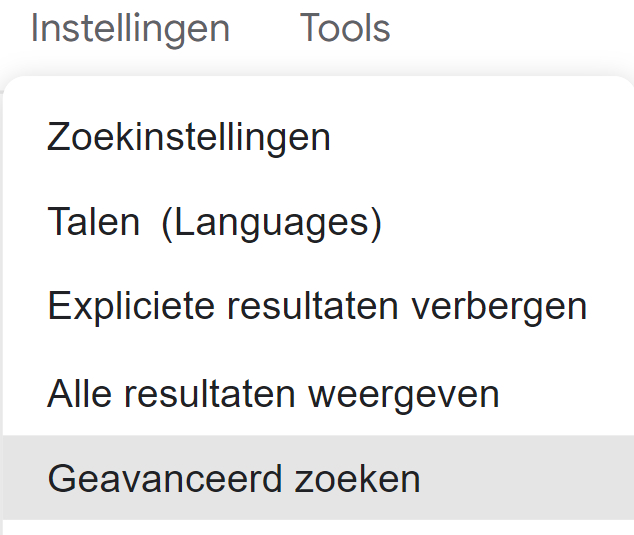
\includegraphics[width=0.6\linewidth]{figurenAuteur/geavanceerd_zoeken.jpg}
\end{center}
Vervolgens opent zich een scherm waarin je heel wat logica kan herkennen.



\section{Propositielogica toegepast op het bewijs uit het ongerijmde}
Het bewijs uit het ongerijmde kan een probleem vormen voor de leerlingen.
De kans daarop is nog groter als de logische stappen in het bewijs niet benadrukt worden.
Voor die stappen gebruiken we een wet uit de propositielogica.

\tussentitel{Wet van de uitgesloten derde}
De wet van de uitgesloten derde klinkt vrij imposant, maar komt in symbolen gewoon neer op $p \lor \lnot p$.
Deze wet kwam reeds aan bod in paragraaf 4.
Als we deze uitspraak interpreteren, staat er simpelweg dat iedere uitspraak $p$ waar of niet waar is.
Anders geformuleerd, als je om één of andere reden weet dat één van de twee opties onmogelijk is, dan weet je dat de andere waar zal zijn.
Als je dus in een gedachtenexperiment kan aantonen dat $\lnot p$ voor problemen zorgt, dan kun je uit de wet van de uitgesloten derde besluiten dat $p$ waar is.
Dit brengt ons bij het bewijs uit het ongerijmde.

\tussentitel{Bewijs uit het ongerijmde}
In een bewijs uit het ongerijmde passen we het stappenplan van daarnet toe.
Om $p$ te bewijzen met een bewijs uit het ongerijmde, onderneem je altijd de volgende stappen.
\begin{opsomming}
    \item Stel dat $\lnot p$ waar is.
    \item Werk op deze hypothese verder, dus in één gedachtenexperiment, tot je een contradictie tegenkomt.
    Die contradictie kan verschillende vormen hebben, zoals $0=1$ of $x>0 \land x<0$.
    Intuïtief gezien, is een contradictie een uitspraak die duidelijk onwaar is.
    \item Aangezien $\lnot p$ niet kan (want anders zouden we die contradictie moeten aanvaarden), besluiten we uit de wet van de uitgesloten derde dat $p$ waar moet zijn.
\end{opsomming}
Leerlingen geraken vaak verloren door de laatste overgang.
In zo'n bewijs is de tweede stap vaak de langste, doe je heel veel werk, maar eindig je dan in iets dat totaal niet klopt, namelijk die contradictie.
Dat is echter niet het einde van het bewijs.
Om verwarring te voorkomen is het dus beter om die structuur te benadrukken.
Ook kan het helpen om doorheen de tweede stap continu duidelijk te maken dat je in een gedachtenexperiment aan het werken bent met de voorwaardelijke wijs ``dan zou ...''.\\

Laten we deze structuur duidelijk maken in een klassiek bewijs uit het ongerijmde.
We bewijzen dat er oneindig veel priemgetallen zijn, dus $p=$ er zijn oneindig veel priemgetallen.
\begin{opsomming}
    \item \textbf{Stel dat $\lnot p$ waar is.}\\
    $\lnot p$ betekent dat er niet oneindig veel priemgetallen zouden zijn.
    We werken dus met de hypothese dat er slechts een eindig aantal priemgetallen is.
    \item \textbf{Werk op deze hypothese verder tot de contradictie.}\\
    Als er slechts een eindig aantal priemgetallen zou zijn, dan kunnen we ze nummeren als $p_1,p_2,p_3,\ldots,p_N$.
    Er zouden dus slechts $N$ priemgetallen zijn.
    Beschouw nu $a = p_1\cdot p_2 \cdot p_3 \cdot \ldots \cdot p_N+1$.
    Dan is $a$ niet deelbaar door $p_1,p_2,\ldots,p_N$ want telkens blijft bij deling nog die $+1$ op het einde over.
    Het getal $a$ is ook niet deelbaar door enig ander natuurlijk getal $n \neq a$, want we hebben al alle mogelijke priemfactoren van $n$ gecontroleerd (namelijk de $p_i$'s).
    Hieruit volgt dat $a$ een priemgetal is, maar dat geeft ons een contradictie.
    Onze hypothese zei namelijk dat er slechts $N$ priemgetallen zijn, maar met $a$ erbij hebben we er $N+1$.
    \item \textbf{Aangezien $\lnot p$ niet kan, besluiten we dat $p$ waar moet zijn.}\\
    Onze aanname dat er slechts een eindig aantal priemgetallen is, kan dus niet kloppen.
    Daarom moeten er wel oneindig veel priemgetallen zijn.
\end{opsomming}

\tussentitel{Verschil tussen bewijs uit het ongerijmde en bewijs via contrapositie}
We eindigen deze paragraaf met een kleine toevoeging over het bewijs uit het ongerijmde.
Deze bewijsvorm wordt vaak toegepast op een implicatie $p \Rightarrow q$.
Daarnaast wordt een implicatie ook vaak bewezen door een bewijs via contrapositie.
Deze twee bewijsvormen lijken soms op elkaar, maar er zijn enkele belangrijke verschillen.\\

Het bewijs uit het ongerijmde op een implicatie heeft altijd de volgende stappen.
\begin{opsomming}
    \item Stel dat $\lnot \left(p \Rightarrow q\right)$ waar is.
    Dit is logisch equivalent met het aannemen dat $p \land \lnot q$ waar is.
    Je kunt dit ook zien als het aannemen van twee hypotheses, namelijk $p$ en $\lnot q$.
    \item We werken zoals gewoonlijk verder met die hypotheses tot we een contradictie uitkomen.
    Een mogelijke weg is om in het gedachtenexperiment proberen $\lnot p$ af te leiden, want dan spreekt dat de aanname $p$ tegen.
    Je kunt echter ook een andere contradictie proberen af te leiden, die niet noodzakelijk iets te maken heeft met je hypotheses.
    \item Dan eindigen we zoals gebruikelijk. Aangezien $\lnot \left(p \Rightarrow q\right)$ voor problemen zorgt, moet het wel zo zijn dat $\left(p \Rightarrow q\right)$ waar is.
\end{opsomming}

Vergelijk dit nu met het bewijs via contrapositie.
\begin{opsomming}
    \item We willen $\left(p \Rightarrow q\right)$ bewijzen, maar die formule is logisch equivalent met $\left(\lnot q \Rightarrow \lnot p\right)$.
    We vervangen dus $\left(p \Rightarrow q\right)$ door $\left(\lnot q \Rightarrow \lnot p\right)$.
    \item In de tweede stap bewijzen we de nieuwe implicatie op een directe manier.
    We leiden dus $\lnot p$ af uit de aanname $ \lnot q$.
    Ons doel is dus niet om een contradictie af te leiden zoals bij het bewijs uit het ongerijmde.
    De redenering kan echter heel gelijkaardig lijken aan de tweede stap bij het bewijs uit het ongerijmde, omdat daar een mogelijke contradictie $p \land \lnot p$ is.
    \item Aangezien we $\lnot p$ konden afleiden uit $\lnot q$, hebben we via contrapositie de stelling $p \Rightarrow q$ bewezen.
\end{opsomming}
Er kan verwarring ontstaan tussen de twee bewijzen in de tweede stap.
Bij het bewijs via contrapositie is het noodzakelijk om $\lnot p$ af te leiden en is er geen sprake van een gedachtenexperiment.
Bij het bewijs uit het ongerijmde is er wel sprake van een gedachtenexperiment en proberen we eigenlijk een contradictie af te leiden, die niet noodzakelijk iets te maken heeft met $\lnot p$.
In de praktijk leidt men echter ook bij het bewijs uit het ongerijmde vaak $\lnot p$ af.
Ieder bewijs via contrapositie kan geherformuleerd worden als een bewijs uit het ongerijmde, maar niet omgekeerd.
Tot slot, ook al zijn deze twee bewijsvormen verschillend van elkaar en ook van een rechtstreeks bewijs van $p \Rightarrow q$, ze kunnen samen voorkomen in een groter bewijs dat ze combineert.
Het is dan echter belangrijk om te benadrukken welk gedeelte een gedachte-experiment is.

\section{True, False of ``Unknown''? Voorbij de propositielogica}
In dit gedeelte tonen we een kleine uitbreiding van logicatalen.
Dit is zowel interessant voor de leerkracht die dit leest als de leerling die naar verdieping snakt.
Het behoort echter niet tot de eindtermen.\\

De wet van de uitgesloten derde zegt dat een uitspraak $p$ ofwel waar ofwel niet waar is.
Er zijn echter contexten denkbaar waar die wet niet langer geldt.
Denk maar aan bijvoorbeeld subjectieve uitspraken als ``Wiskunde is leuk!'' of uitspraken waarvan het niet geweten is of ze waar zijn of niet zoals ``De kat in de doos is dood.'' (vooraleer je de doos openmaakt).
In propositielogica worden deze uitspraken niet beschouwd.
Stel dat we echter onze logicataal kunnen uitbreiden met een derde mogelijkheid voor de waarheidswaarde zoals ``nog niet geweten'', hoe zouden onze klassieke logische connectieven er dan uit zien?
Dit brengt ons tot de zogenaamde driewaardige logica.\\

In dit gedeelte gebruiken we de notatie $T$ van `True' voor waar, $F$ van `False' voor vals en $U$ van `Unknown' voor onbepaald om echt duidelijk te maken dat het over een verschillende logicataal gaat.
Voor de definitie van de logische connectieven zullen we ervoor zorgen dat ze zich met de waarden $T$ en $F$ net zoals vroeger gedragen.
Het is enkel als er een $U$ in het spel is, dat we iets nieuws zullen moeten bedenken.
De logische negatie wordt in iedere logicataal met drie waarden als volgt gedefinieerd:
\begin{center}
\begin{tabular}{c|c}  
$p$ & $\lnot p$\\
\hline
$T$ & $F$\\
$U$ & $U$\\
$F$ & $T$
\end{tabular}
\end{center}
De negatie van $U$ is dus opnieuw $U$.
Als je niet weet of een uitspraak waar of vals is, dan weet je ook niets over de negatie van die uitspraak.
In de oefening bekijken we de andere connectieven.\\

Zijn er ook praktische redenen om een logica met drie mogelijke waarheidswaarden te gebruiken?
Ja!
Dit heeft namelijk concrete toepassingen in statistische analyses op datasets en software die databases manipuleert.\\

Stel dat je een analyse doet over de efficiëntie van een bepaalde medicatie.
Tijdens je onderzoek wil je specifiek bekijken hoe de medicatie werkt op rokers. Je wilt dus je dataset filteren tot bijvoorbeeld alle rokers die niet gestorven zijn na het innemen van de medicatie.
De programmeertaal die je daarvoor gebruikt, zal kijken welke observaties de formule ``de geobserveerde persoon rookt $\land \lnot$ de geobserveerde persoon is gestorven'' waar maken.
Hoewel de informatie of je rookt of niet, en of je gestorven bent of niet op het eerste zicht binaire variabelen lijken, is er in de praktijk nog een derde mogelijkheid.
Die derde mogelijkheid is dat je het niet weet!
Vele datasets zijn namelijk niet volledig, en er zal op verschillende plaatsen ``NA'' (van ``Not Available'') te vinden zijn.
Dit komt overeen met onze $U$.
Dit kan bijvoorbeeld voorkomen als je een dataset hebt die opgesteld is in verschillende landen, waarbij één land wel registreerde wie er rookte (dan staat er $T$ of $F$), maar een ander land niet (en die mensen dus $U$ zullen hebben bij de variabele over roken).
Hoe we de logische connectieven definiëren zal dus bepalen of je liever mensen wegfiltert of toch meeneemt van wie je niet weet of ze roken.
Laat ons in de oefening een concrete driewaardige logica bestuderen.
Daar zul je ook merken dat er keuzes in de definitie zijn.\\


\end{multicols}
\beginwerktekst{Definiëren van logische connectieven in een driewaardige logica}
% ge kunt eventueel één connectief op verschillende manier definiëren om het aan te tonen?

In deze oefening zullen we de logische conjunctie definiëren als er drie mogelijke waarheidswaarden zijn, True, False en Unknown. De 9 mogelijkheden voor twee uitspraken kunnen we in plaats van onder elkaar te zetten, ook in een waarheidstabel met rijen en kolommen plaatsen.
Waar er nu vraagtekens staan, zal de definitie van de conjunctie komen.
De waarde van $F \land U$ zal dus in de vierde rij en derde kolom komen.

\begin{center}
\begin{tabular}{c|c|c|c}  
$\land$ & $T$ & $U$ & $F$\\
\hline
$T$ & ?? & ?? & ??\\
\hline
$U$ & ?? & ?? & ??\\
\hline
$F$ & ?? & ?? & ??
\end{tabular}
\end{center}

Bij de meeste opgaven zijn er verschillende manieren om te antwoorden.

\begin{werktekstoef}


\item{We willen dat de conjunctie zich gedraagt als vroeger. Je kunt dus al de cellen aanvullen, waar er geen sprake is van $U$.}\\

\emph{Dit is in principe een keuze, maar dit wordt in alle driewaardige logica's wel zo gedaan. We krijgen dus in de eerste stap de volgende tabel:
\begin{center}
\begin{tabular}{c|c|c|c}  
$\land$ & $T$ & $U$ & $F$\\
\hline
$T$ & $T$ & ?? & $F$\\
\hline
$U$ & ?? & ?? & ??\\
\hline
$F$ & $F$ & ?? & $F$
\end{tabular}
\end{center}
}

\item{Daarnaast willen we ook dat de conjunctie commutatief is. Dit betekent dat $p \land q$ dezelfde waarde heeft als $q \land p$. Wat betekent het om commutatief te zijn in onze tabel?}\\

\emph{De commutativiteit betekent bijvoorbeeld dat $U \land T$ dezelfde waarde moet krijgen als $T \land U$.
De tabel moet dus symmetrisch zijn rond de diagonaal van linksboven naar rechtsbeneden.
}

\item{Vervolgens kiezen we ervoor om de $\land$ streng te maken. Dit betekent dat van zodra de conjunctie kan, hij zal proberen iets als $F$ te bestempelen. Zijn er cellen die al zeker een $F$ kunnen krijgen?}\\

\emph{We kunnen al invullen dat $U \land F$ en $F \land U$ de waarde $F$ hebben.
We weten (nog) niet wat $U$ is, want het is `Unknown', maar dat maakt niet zo veel uit.
Als er al één van de uitspraken vals is, dan weten we zeker dat de conjunctie vals zal zijn.
}

\item{Vul nu de rest van de tabel aan door te redeneren zoals daarnet. De waarde $U$ betekent ``Unknown'', je weet niet of ze waar of vals is.}\\

\emph{We moeten nog maar twee combinaties kiezen.
$U \land U$ is zeker $U$.
Als je over beide uitspraken niet weet of ze waar zijn, dan weet je het ook niet over de conjunctie.
Verder is $T \land U$ ook $U$ om gelijkaardige reden.
We krijgen:
\begin{center}
\begin{tabular}{c|c|c|c}  
$\land$ & $T$ & $U$ & $F$\\
\hline
$T$ & $T$ & $U$ & $F$\\
\hline
$U$ & $U$ & $U$ & $F$\\
\hline
$F$ & $F$ & $F$ & $F$
\end{tabular}
\end{center}
}

\item{We zouden de $\lor$ helemaal losstaand kunnen definiëren van de $\land$, maar dat doen we liever niet. In propositielogica hebben we de wetten van De Morgan die onder andere zeggen dat $\lnot \left(\lnot p \land \lnot q\right)$ altijd dezelfde waarde heeft als $p \lor q$.
Definieer de $\lor$ zodat aan die wet voldaan is.}\\

\emph{Hiervoor kun je de (verticale) waarheidstabel opstellen van $\lnot \left(\lnot p \land \lnot q\right)$.
Daaruit kun je meteen de waarden van $p \lor q$ aflezen.
\begin{center}
\begin{tabular}{c|c|c|c|c|c}  
$p$ & $q$ & $\lnot p$ & $\lnot q$ & $\lnot p \land \lnot q$ & $\lnot \left(\lnot p \land \lnot q\right)$\\
\hline
$T$ & $T$ & $F$ & $F$ & $F$ & $T$\\
$T$ & $U$ & $F$ & $U$ & $F$ & $T$\\
$T$ & $F$ & $F$ & $T$ & $F$ & $T$\\
$U$ & $T$ & $U$ & $F$ & $F$ & $T$\\
$U$ & $U$ & $U$ & $U$ & $U$ & $U$\\
$U$ & $F$ & $U$ & $T$ & $U$ & $U$\\
$F$ & $T$ & $T$ & $F$ & $F$ & $T$\\
$F$ & $U$ & $T$ & $U$ & $U$ & $U$\\
$F$ & $F$ & $T$ & $T$ & $T$ & $F$
\end{tabular}
\end{center}
wat ons in de andere waarheidstabel geeft:
\begin{center}
\begin{tabular}{c|c|c|c}  
$\lor$ & $T$ & $U$ & $F$\\
\hline
$T$ & $T$ & $T$ & $T$\\
\hline
$U$ & $T$ & $U$ & $U$\\
\hline
$F$ & $T$ & $U$ & $F$
\end{tabular}
\end{center}
Je zou ook via intuïtieve redeneringen op de betekenis van $U$ de tabel van $\lor$ kunnen opstellen, en achteraf controleren of aan de wet voldaan is.
}

\item{Als je nu nog de $\Rightarrow$ definieert, kan je jezelf als klaar beschouwen. We kunnen er opnieuw voor kiezen om een wet uit de propositielogica over te hevelen naar onze driewaardige logica. In propositielogica is namelijk $p\Rightarrow q$ logisch equivalent met $\lnot p \lor q$. Definieer de $\Rightarrow$ hier zodat nog steeds aan die wet voldaan is.}\\

\emph{Je kunt deze vraag op verschillende manieren oplossen.
Je kunt redeneren op de intuïtieve betekenis van $U$ zoals bij de derde vraag.
Je kunt een waarheidstabel opstellen van de relevante wet zoals bij de vijfde vraag.
We focussen op het spiegelen/manipuleren van de tabel zoals bij de tweede vraag. Hieronder staat de tabel van $p \lor q$, wat dicht in de buurt is van $\lnot p \lor q$.
\begin{center}
\begin{tabular}{c|c|c|c}  
$\lor$ & $T$ & $U$ & $F$\\
\hline
$T$ & $T$ & $T$ & $T$\\
\hline
$U$ & $T$ & $U$ & $U$\\
\hline
$F$ & $T$ & $U$ & $F$
\end{tabular}
\end{center}
Om de tabel van $\lnot p \lor q$ te verkrijgen, moeten we er nog de negatie in brengen.
De negatie betekent in de tabel dat je moet spiegelen, want $U$ blijft zichzelf en $T$ en $F$ wisselen van plaats.
Voor de tabel van $ p \lor \lnot q$ moet je verticaal spiegelen, voor $\lnot p \lor q$ horizontaal.
We krijgen op die manier dus onmiddellijk de waarheidstabel van $\Rightarrow$.
\begin{center}
\begin{tabular}{c|c|c|c}  
$\Rightarrow$ & $T$ & $U$ & $F$\\
\hline
$T$ & $T$ & $U$ & $F$\\
\hline
$U$ & $T$ & $U$ & $U$\\
\hline
$F$ & $T$ & $T$ & $T$
\end{tabular}
\end{center}
Merk op dat deze tabel duidelijk niet symmetrisch is rond de diagonaal van linksboven naar rechtsbeneden.
Dit bevestigt dat $\Rightarrow$ niet commutatief is.
}

Proficiat!
Je hebt een logisch systeem opgesteld dat beter overweg kan met de onzekerheden van het leven!
\end{werktekstoef}  
\eindewerktekst



\stopcontents[mainsections]			        % altijd laten staan, opsomming in inhoudstafel enkel tot loep beperken


% bronnen toevoegen (hieronder staan enkele voorbeelden)
\begin{bronnen}
\item Durand-Guerrier, V., Boero, P., Douek, N., Epp, S. S., Tanguay, D. (2011). Examining the role of logic in teaching proof. in \emph{Proof and proving in mathematics education (pp. 369-389)}. Springer, Dordrecht.
\item Milbouw, L. \textit{Cursustekst logica}. UAntwerpen.
\item op den Brouw, J. (2020). \textit{Digitale techniek. Een inleiding in het ontwerpen van digitale systemen. Deel 1}. Den Haag. Geraadpleegd via  https://ds.opdenbrouw.nl/inldig/dictaat\textunderscore inldig.pdf
\item Roelens, M., Tytgat, P. (2011). Logica. \emph{Uitwiskeling 27/2}.
\item Roodhardt, A., Doorman, M. (2009). \textit{Logisch redeneren}. Lesmateriaal voor experimenten Wiskunde C in het kader van het project commissie toekomst wiskunde-onderwijs (cTWO) voor de vernieuwing van wiskunde in de tweede fase per 2011 (www.ctwo.nl).
\item Wason, P. C., Johnson-Laird, P. N. (1972). \emph{Psychology of Reasoning: Structure and Content}. Cambridge, MA: Harvard University Press.


\end{bronnen}
